\documentclass[12pt,reqno]{amsart}
%\documentclass{amsart}
\renewcommand{\labelenumi}{(\alph{enumi})}



\setlength{\textwidth}{6in}
\setlength{\textheight}{8.5in}
\hoffset=-0.5in

\usepackage{diagrams}

\usepackage[utf8]{inputenc}
\usepackage{graphicx}
\usepackage{amssymb}
\usepackage{amsmath}
\usepackage{epstopdf}
\usepackage{amsthm}
%\usepackage{xypic}
\usepackage{enumerate}
%\usepackage{sidenotes}

%\usepackage{fourier}
%\usepackage{a4wide}


\newtheorem{definition}{Definition} 
\numberwithin{definition}{section}
\newtheorem{proposition}[definition]{Proposition} 
\newtheorem{theorem}[definition]{Theorem} 
\newtheorem{lemma}[definition]{Lemma} 
\newtheorem{corollary}[definition]{Corollary}
\newtheorem{conjecture}[definition]{Conjecture}
\newtheorem{question}[definition]{Question}
\newtheorem{claim}[definition]{Claim}
\newtheorem{fact}[definition]{Fact}
\newtheorem{remark}[definition]{Remark}
\newtheorem{wedgelemma}[definition]{Wedge Lemma} 
\newtheorem{construction}[definition]{Construction}

\theoremstyle{definition}
\newtheorem{example}[definition]{Example}



\newcommand{\lo}{\preceq}
\newcommand{\rar}{\rightarrow}
\newcommand{\rAr}{\Rightarrow}
\newcommand{\lrAr}{\Leftrightarrow}
\newcommand{\RR}{\mathbb{R}}
\newcommand{\NN}{\mathbb{N}}
\newcommand{\QQ}{\mathbb{Q}}
\newcommand{\ZZ}{\mathbb{Z}}
\newcommand{\AAA}{\mathcal{A}}
\newcommand{\FFF}{\mathcal{F}}
\newcommand{\HHH}{\mathcal{H}}
\newcommand{\NNN}{\mathcal{N}}
\newcommand{\SSS}{\mathcal{S}}
\newcommand{\K}{\mathbf{K}}
\renewcommand{\L}{\mathbf{L}}
\newcommand{\U}{\mathbf{U}}
\newcommand{\V}{\mathbf{V}}
\newcommand{\X}{\mathbf{X}}
\newcommand{\Rat}{\operatorname{Rat}}
\newcommand{\ehr}{\operatorname{ehr}}
\newcommand{\dist}{\mathsf{dist}}
\newcommand{\sgn}{\mathrm{sgn}}
\newcommand{\sprod}[2]{\langle #1, #2 \rangle}
\newcommand{\mspan}{\operatorname{span}}
\renewcommand{\dim}{\mathsf{dim}\ }
\newcommand{\inter}{\mathsf{int}\ }
\newcommand{\median}{\mathrm{median}\ }
\DeclareMathOperator*{\argmin}{arg\,min}

\newcommand{\defn}[1]{\emph{#1}}
\newcommand{\norm}[1]{|| #1 ||}

\newcommand{\Glat}{G^{\operatorname{lat}}}
\newcommand{\Gdep}{G^{\operatorname{dep}}}
\newcommand{\Gfine}{G^{\operatorname{fine}}}
\newcommand{\Gfinem}{G^{\operatorname{fine*}}}

\newcommand{\FD}{\mathcal{F}}

\newcommand{\path}{\operatorname{path}}
\newcommand{\reldep}[2]{{#1} \longrightarrow {#2}}
\newcommand{\reldepi}[3]{{#1} \overset{#2}{\longrightarrow} {#3}}
\newcommand{\shift}[2]{\rightarrow(#1,{#2})}
\newcommand{\shiftw}[3]{\overset{#1 \cdot #2}{\longrightarrow} {#3}}

\newcommand{\conv}{\operatorname{conv}}
\newcommand{\cone}{\operatorname{cone}}
\newcommand{\lev}{\operatorname{lev}}
\newcommand{\Lev}{\operatorname{Lev}}
\renewcommand{\deg}{\operatorname{deg}}
\renewcommand{\dim}{\operatorname{dim}}
\renewcommand{\min}{\operatorname{min}}
\renewcommand{\max}{\operatorname{max}}
\newcommand{\fract}{\operatorname{frac}}
\newcommand{\integ}{\operatorname{int}}
\newcommand{\relint}{\operatorname{relint}}

\newcommand{\twin}{\mathsf{twin}}
\newcommand{\hull}{\mathsf{hull}}
\newcommand{\diam}{\mathsf{diam}}
\newcommand{\choice}[1]{\left\{ \begin{array}{ll} #1 \end{array} \right.}
\newcommand{\floor}[1]{\lfloor {#1} \rfloor}
\newcommand{\ceil}[1]{\lceil {#1} \rceil}
\newcommand{\mset}[2]{ \left\{ #1 \; \middle| \; #2 \right\}}
\newcommand{\lk}{\mathsf{lk}}
\newcommand{\sd}{\mathsf{sd}}
\newcommand{\Pa}{\mathrm{P}}
\newcommand{\dotcup}{\ensuremath{\mathaccent\cdot\cup}}
\newcommand{\Hom}{\mathrm{ Hom}}
\newcommand{\om}{\omega}

%% IMPORTANT OBJECTS FOR THIS ARTICLE

\newcommand{\ncM}{\mathcal{M}}
\newcommand{\ncL}{\mathcal{L}}

% we are working with (at least) four different "Braid triangulations"
\newcommand{\T}{T} % generic symbol for the triangulation
\newcommand{\Tn}{T_n} % generic symbol for the triangulation with dimension
\newcommand{\TRn}{\T_{\RR^n}} % the braid triangulation of space
\newcommand{\TS}{\T_{S^{n-2}}} % the braid triangulation of the sphere (i.e. the Coxeter complex)
\newcommand{\TP}{\T_{\RR^n_{> 0}}} % the braid triangulation of the positive orthand
\newcommand{\TC}{\T_{(0,1)^n}} % the braid triangulation of the cube

\newcommand{\allow}{\operatorname{Allow}} % the allowed subcomplex
\newcommand{\forb}{\operatorname{Forb}} % the forbidden subcomplex
% variants of allowed and forbidden subcomplexes for different triangulations
\newcommand{\allowRn}{\allow_{\RR^n}} % the braid triangulation of space
\newcommand{\allowS}{\allow_{S^{n-2}}} % the braid triangulation of the sphere (i.e. the Coxeter complex)
\newcommand{\allowP}{\allow_{\RR^n_{> 0}}} % the braid triangulation of the positive orthand
\newcommand{\allowC}{\allow_{(0,1)^n}} % the braid triangulation of the cube
\newcommand{\forbRn}{\forb_{\RR^n}} % the braid triangulation of space
\newcommand{\forbS}{\forb_{S^{n-2}}} % the braid triangulation of the sphere (i.e. the Coxeter complex)
\newcommand{\forbP}{\forb_{\RR^n_{> 0}}} % the braid triangulation of the positive orthand
\newcommand{\forbC}{\forb_{(0,1)^n}} % the braid triangulation of the cube


\newcommand{\comment}[1]{\textsf{\footnotesize #1}}


\begin{document}
\title{Scheduling Problems}
\author{Felix Breuer, Caroline J. Klivans}



\begin{abstract}{(Placeholder basically from my talk abstract) We introduce new families of polynomials associated to scheduling problems.  Our starting point is the consideration of counting functions which enumerate the number of solutions to certain scheduling problems.  These scheduling problems arise naturally in the context of the normal fan of a related polytope.  This approach creates a connection to Erhart theory and quasisymmetric functions which allows us to establish polynomiality of the counting functions easily. Moreover, from these perspectives we establish bounds on the coeffiecients of the polynomials, reciprocity theorems and nonnegativity of certain basis exapansions. 

This approach includes certain classic polynomials arising in geometric combinatorics such as the chromatic polynomial, but also polynomials that do not satisfy contraction/deletion and hence are not generally Tutte invariants.  For example, we define the arboricity polynomial which counts the number of matroid covers with a fixed number of independent sets.}
\end{abstract}
\maketitle


\tableofcontents

%%%%%%%%%%%%%%%%%%%%%%%%%%%%%%%%%
\section{Introduction}
%%%%%%%%%%%%%%%%%%%%%%%%%%%%%%%%%



A \defn{scheduling problem} $S$ on $d$ items is given by a boolean formula $\phi$ over atomic formulas $\omega_i\leq \omega_j$ for $i,j\in[d]$. A \defn{$k$-schedule} solving $S$ is a function $\omega:[n]\rightarrow[k]$ such that $\phi(\omega)$ is true.

* Constraint satisfaction problem.



\section{Motivating examples}

%*** Illustrate the overall ideas and methods through a motivating example(s).  Choose examples that are not the 'prettiest', namely that would not fall under other methods, and do not just do the chromatic polynomial. ****

%% Given a graph, most naturally we consider the graphical arrangement,
%% the subarrangement of the Braid arrangement given by hyperplanes
%% indexed by edges in the graph.

%% Given a matroid, we consider the matroid polytope formed by the convex
%% hull of the support vectors of bases.  The normal fan of the matroid
%% polytope is refined by the Braid arrangement, but this fan and the
%% graphical arrangement are not the same.  

%% We considered the very special case of graphical matroids.  Matroids
%% whose bases correspond to spanning trees of a graph.  Take the
%% \emph{matroid polytope} approach to a graphical matroid.  What integer
%% points / weight classes / relative orderings are induced?  We saw more
%% complicated 'rules', for example:\\

$x_1 \neq x_2$ if $x_3 \geq x_1$.  But $x_1 = x_2$ is ok if $x_3 < x_1$.\\

We interpreted this as {\bf{scheduling}} of tasks.  Tasks $x_1$ and
$x_2$ can be performed  at the same time only if $x_3$ happens first.

\begin{figure}[h]
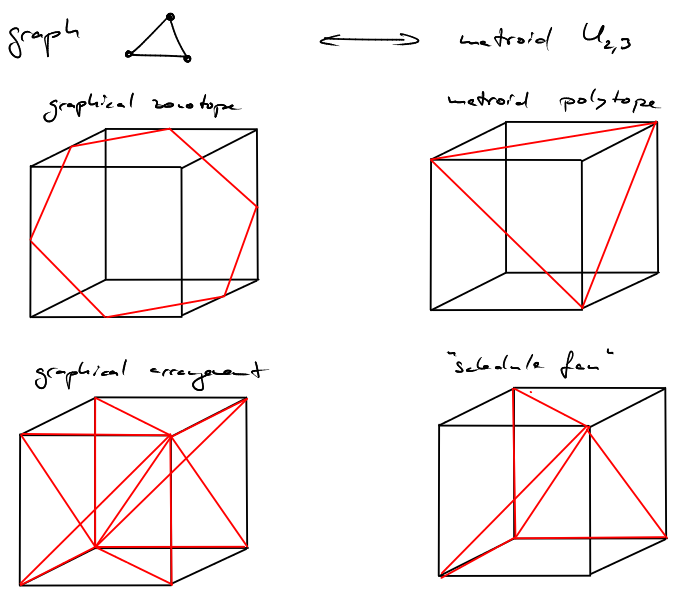
\includegraphics[width=13cm]{graph-matroid}
\caption{Difference between graph construction and graphical matroid construction.}
\end{figure}


\begin{figure}[h]
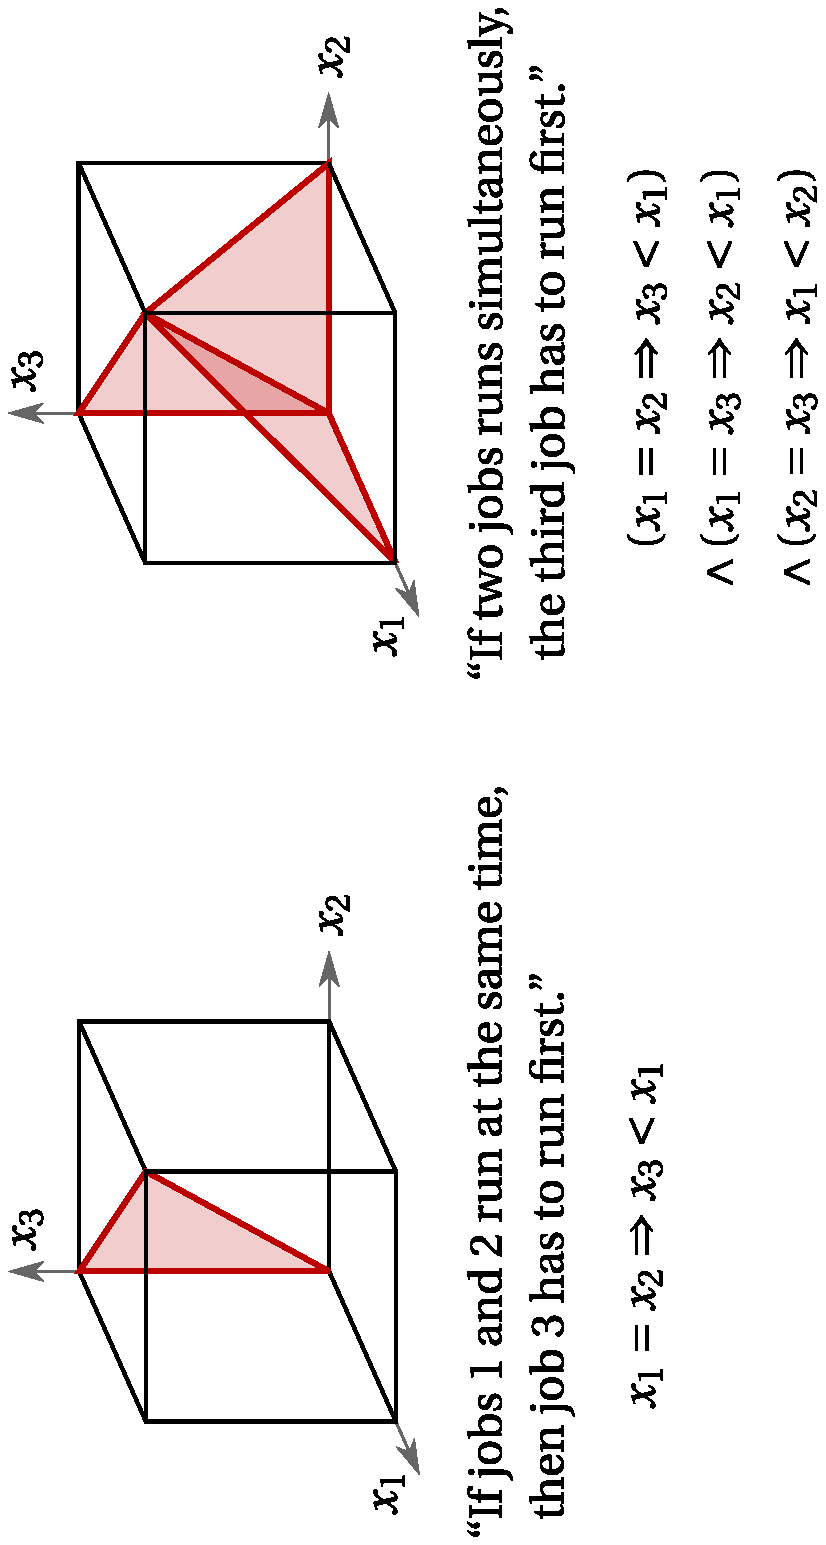
\includegraphics[width=13cm]{schedule}
\caption{Two "scheduling arrangements".}
\end{figure}

One of the staples of geometric methods in combinatorics is to interpret a monomial as an integer point in space. The standard construction is to view a monomial in commuting variables $x_1^{a_1}x_2^{a_2}\cdot\ldots\cdot x_d^{a_d}$ as the point $(a_1,a_2,\ldots,a_d)\in\ZZ^d$. To translate quasisymmetric functions in non-commuting variables into a geometric setting, we need to use a different construction, however. Here we associate to a monomial $x_{i_1} x_{i_2} \cdot \ldots \cdot x_{i_d}$ the point $(i_1,\ldots,i_d)\in \ZZ^d$. For example $x_2x_1x_3$ becomes $(2,1,3)\in\ZZ^3$. That is, the entries of the vector are given by the \emph{indices} of the monomial, as opposed to the exponents. This works because we are working with non-commuting variables here, so that the factors $x_i$ appear in a fixed order.

Quasisymmetric functions in non-commuting variables are going to be introduced in detail in Section~\ref{sec:prelim-qsym}. For now, we just consider the examples in Figure~\ref{fig:cone}. When viewed through the geometric lens explained above the infinite formal sum $\sum_{0<i_3<i_1<i_2} x_{i_1}x_{i_2}x_{i_3}$ in the non-commuting variables $x_1,x_2,x_3,\ldots$, corresponds to the set of integer points $z\in\ZZ^3$ with $0<z_3<z_1<z_2$, that is, the set of integer points in the relative interior of the cone generated by vectors $e_2,e_1+e_2$ and $e_1+e_2+e_3$. If we turn one of the two inequalities into equalities, i.e., we pass to the sums $\sum_{0<i_3<i_1 = i_2} x_{i_1}x_{i_2}x_{i_3}$ and $\sum_{0<i_3=i_1<i_2} x_{i_1}x_{i_2}x_{i_3}$, we obtain two facets of this cone. More precisely, we obtain the set of lattice points in the relative interiors of the cones $\cone_\ZZ(e_1+e_2,e_1+e_2+e_3)$ and $\cone_\ZZ(e_2,e_1+e_2+e_3)$, respectively.

** In Figure 2, we should replace implies with AND to keep everything a Boolean formula over pairwise comparisions. 

\section{Preliminaries: Ehrhart Theory}

%*** cjk: We will need a Preliminaries: Ehrhart Theory section.  I don't know if it should go before or after the next one.  I have given a minimal introduction to the coxeter complex (of type A), quasisymmetric functions and NCQSym.  Telling a very narrow narrative so as to think about these objects specifically the way we want to use them. ***

Consider a (bounded) set $X\subset \RR^d$. The \emph{Ehrhart function} 
\[
  \ehr_X:\ZZ_{> 0}\rar\ZZ_{\geq 0}
\]
of $X$ counts the number of integer points in integer dilates of $X$, i.e., 
\[
  \ehr_X(k) = \#\ZZ^d \cap k\cdot X
\]
for any positive integer $k$. Ehrhart's theorem states that if $X$ is a polytope whose vertices have integer coordinates, then the Ehrhart function $\ehr_X$ of $X$ coincides with a polynomial, called the Ehrhart polynomial of the polytope. We call polytopes whose vertices have integer coordinates \emph{integral} or \emph{lattice polytopes}. Two polytopes in $\RR^d$ are \emph{lattice equivalent} if there is an affine automorphism $\phi$ of $\RR^d$ with $\phi(P)=Q$ which induces a bijection on the integer lattice $\ZZ^d$.

The most important example for our purposes are the Ehrhart polynomials of simplices. The $d$-dimensional \emph{standard simplex} $\Delta^d$ is the convex hull of the standard unit vector $e_1,\ldots,e_d\in\RR^{d+1}$, i.e.,
\begin{eqnarray*}
  \Delta^d &=& \mset{x\in\RR^{d+1}}{\sum x_i =1, x_1 \geq 0, \ldots, x_{d+1} \geq 0} \\
  &=& \mset{\sum_{i=1}^{d+1} \lambda_i e_i\in\RR^{d+1}}{\sum_{i=1}^{d+1} \lambda_i = 1, \lambda_i\geq 0, }.
\end{eqnarray*}
Its Ehrhart polynomial is given by a binomial coefficient
\[
  \ehr_{\Delta^d}(k) = \binom{k+d}{d} = \frac{1}{d!} (k+d)\cdot (k+d-1) \cdot \ldots \cdot (k+1)
\]
which is a polynomial of degree $d$ in the variable $k$. An integral simplex is \emph{unimodular} if it is lattice equivalent to a standard simplex, whence all unimodular simplices of the same dimension have the same Ehrhart polynomial. Note that all faces of a unimodular simplex are themselves unimodular simplices.

Ehrhart polynomial of unimodular simplices arise naturally from the study of scheduling problems. Consider the following scheduling problem: "Schedule two jobs, 1 and 2, such that job 2 starts after or at the same time as job 1." Suppose jobs can be run in discrete time slots, numbered $0$ through $k$. A feasible schedule is a pair of integer numbers $0\leq x_1,x_2 \leq k$ such that $x_1 \leq x_2$. The feasible schedules are precisely the integer points $x=(x_1,x_2)$ contained in the $k$-th dilate of the unimodular simplex $\conv(0,e_2,e_1+e_2)$. Therefore, if we let the deadline $k$ vary, the number of feasible schedules is given by the Ehrhart polynomial of a 2-dimensional unimodular simplex, $\ehr_{\Delta^d}(k)=\binom{k+2}{2}$.

What if, instead, we require job 2 to run strictly after job 1? In this case, feasible schedules are integer points $x\in\ZZ^2$ such that $0\leq x_1,x_2 \leq k$ and $x_1 < x_2$. The strict inequality gives rise to a \emph{half-open simplex}: The $d$-dimensional standard simplex $\Delta^d_i$ with $i$ open faces is defined just as standard simplex above, except that $i$ of the inequalities are strict. More precisely
\[
    \Delta^d_i = \mset{x\in\RR^{d+1}}{\sum x_i =1, x_1 \geq 0, \ldots, x_i > 0, x_{i+1} \geq 0, x_{d+1} \geq 0}.
\]
For every face of the standard simplex that we open, we have to shift the Ehrhart polynomial by one:
\[
  \ehr_{\Delta^d_i}(k) = \binom{k+d-i}{d}.
\]
In particular, the open simplex $\Delta^d_{d+1} = \relint{\Delta^d}$ has Ehrhart polynomial $\ehr_{\Delta^d_{d+1}}(k) = \binom{k-1}{d}$. The feasible schedules in the example mentioned above therefore correspond to the integer points in the $k$-th dilate of a $2$-dimensional unimodular simplex with $1$ open face, and their number is $\ehr_{\Delta^2_1} = \binom{k+1}{2}$.

But half-open simplices do not suffice to capture all scheduling problems. Consider the following variation of our running example: "Schedule two jobs, 1 and 2, such that job 2 starts strictly after job 1. However, if job 1 starts immediately, then both can run at the same time." The exception that both jobs may run simultaneously if they are started immediately adds one point to our half-open simplex: the origin $(0,0)$. The resulting set is no longer a half-open simplex. In fact, it is not even the set-theoretic difference of two closed polytopes. In order to capture this type of geometric object, we work with partial polytopal complexes.

A \emph{polytopal complex} $K$ is a finite set of polytopes in some $\RR^d$ such that $K$ is closed under taking faces and the intersection of any two polytopes in $K$ is a face of both. A polytopal complex is \emph{integral} if all vertices have integer coordinates. We define the \emph{relative interior} of a polytope to be the interior of the polytope taken with respect to its affine hull, so that, for example, the interior of a 2-dimensional triangle in 3-space is the triangle minus its edges and vertices. This definition is important because of the following property: The union of all faces of a polytopal complex is equal to the \emph{disjoint} union of the relative interiors of all faces. For example, a triangle is equal to the open 2-dimension region, plus the open line segments corresponding to the edges, plus the vertices (which are open in their 0-dimensional affine hull). This observation implies that the Ehrhart function of a polytopal complex is just the sum of all Ehrhart functions of the relative interiors of all faces.

Now, how about our half-open triangle with that one extra point? It can be written as the disjoint union of the open 2-dimensional region, the open line segments corresponding to the two closed edges, and the two vertices that we want to include: the origin and $e_2$. However, we exclude the open line segment from 0 to $e_1+e_2$ and the vertex $e_1+e_2$ from the union. This idea of taking the relative interiors of just some of the faces of a polytopal complex gives rise to the notion of a partial polytopal complex. A \emph{partial polytopal complex} is a subset of the faces of a polytopal complex; in particular, partial polytopal complex is not closed under taking faces. The \emph{support} $|K|$ of a partial polytopal complex $K$ is the union of the relative interiors of all faces contained in $K$.

It will be useful to also consider the following alternative definition of a partial polytopal complex. We call the relative interior of a polytope $P$ an \emph{open polytope}. The \emph{faces of an open polytope} are the faces of its closure. By extension, we define the \emph{closure} of any set of open polytopes as the set of all faces of these polytopes. A \emph{partial polytopal complex} $K$ is now any set of open polytopes whose closure $\bar{K}$ is a polytopal complex. Note that indeed $\bar{|K|}=|\bar{K}|$, i.e., the closure of the support is the support of the closure. We will at certain points need to distinguish between the faces of $K$ and the faces of $\bar{K}$. For example, let $K$ be the interior of a triangle together with one of its vertices. In this case, $K$ will have just two faces: the open triangle and the vertex. However, we will have recourse to refer to the other faces of the (closed) triangle as well. These make up the faces of $\bar{K}$.

The Ehrhart function of a partial polytopal complex is the Ehrhart function of its support. If the complex is integral it is straightforward to show that the Ehrhart function is again a polynomial. In the example of half-open simplex with the extra point, we can thus observe that its Ehrhart function is $\binom{k+1}{2} + 1$.

This motivates the following observation: If $K$ is a partial simplicial complex in which all vertices are integral and all simplices are unimodular. Then, the Ehrhart function $\ehr_K$ satisfies
\[
  \ehr_K(k) = \sum_{i=0}^d f_i^* \binom{k-1}{i}
\]
where $d$ is the dimension of $K$ and $f_i^*$ denotes the number of $i$-dimensional faces in $K$. As it turns out the polynomials $\binom{k+d-i}{d}$ form a basis of the space of polynomials of degree at most $d$. Thus every Ehrhart polynomial can be written in the above form and the $f_i^*$ are coefficients of the polynomial with respect to this binomial basis. Intuitively, the coefficients $f_i^*$ count how many unimodular simplices of dimension $i$ the complex contains. This will be made precise in Section~\ref{sec:scheduling-problems}.

\section{Preliminaries: Coxeter Complexes, QSym and NCQsym}
\label{sec:prelim-qsym}

\subsection{Quasisymmetric functions}
A quasisymmetric function is a formal power series in infintely many
variables which has bounded degree and is shift invariant.  Namely, for
a composition $\alpha$, the coefficients of all terms
$x_{i_1}^{\alpha_1}x_{i_2}^{\alpha_2} \cdots x_{i_k}^{\alpha_k}$,
running over all possible $k$-tuples $\{i_1 < i_2 < \ldots < i_k \}$, are
the same.


The monomial quasisymmetric function indexed by the composition $\alpha$ is 
$$M_{\alpha} := \sum_{1 \leq i_1 < i_2 < \ldots < i_k}
x_{i_1}^{\alpha_1} \ldots x_{i_k}^{\alpha_k}.$$  One may equivalently
define quasisymmetric functions as any series which may be written as a
linear combination of monomial quasisymmetric functions.

%We will be particularly interested in quasisymmetric functions that have appeared in connection to 
%Quasisymmetric functions have been recent begun to appear in connection with 
%% ** cjk: could include here a discuss of quasisymmetric functions that have
%% been considered in 'geometric combinatorics', chromatic, matroid,
%% generalized permutahedra **  Problem is that with these three, the first two are cases of the third.


%% , i.e. the
%% monomial quasisymmetric functions form a basis for the ring of all
%% quasisymmetric functions.  Clearly any collection of
%% compositions of $n$ gives rise to a quasisymmetric function simply by
%% taking the sum of monomial quasisymmetric functions indexed by
%% compositions in the collection.

\subsection{The Coxeter Complex of Type A}
Scheduling problems naturally arise at the level of ordered set partitions instead of
compositions.  The correct setting for us will be the algebra of  
quasisymmetric functions in non-commuting variables, NCQSym.

Before defining these classes, we motivate working with ordered set
partitions by considering the Coxeter complex of type $A$.  Many of
our arguments will be of a geometric nature concerning the structure
of this complex.


An \emph{ordered set partition} or \emph{set composition} $\Phi \vDash
[n]$ is a sequence of sets $(\Phi_1, \Phi_2, \ldots, \Phi_k)$ such that $\forall
i,j$, $ \Phi_i \cap \Phi_j = \empty$ and $\cup_i \Phi_i = [n]$.  The $\Phi_i$ are the
blocks of the ordered set partition and we will often use the notation
$\Phi_1| \Phi_2| \ldots| \Phi_k$.  Note that within each block, elements are
not ordered, so the ordered set partition $13|4|2 \vDash [4]$ is the
same as $31|4|2$.

%**fb: Are the $F^i$ allowed to be empty?** No.


The Braid arrangement $\mathcal{B}_n$ is the hyperplane arrangement in
$\mathbb{R}^n$ consisting of hyperplanes $x_i = x_j$ for all $i,j \in [n]$.
Note that this arrangement is central, that is all hyperplanes contain
the origin, it is also non-essential, that is the collection of
normals to the hyperplanes do not span all of $\mathbb{R}^n$.  The
hyperplanes have a common intersection equal to the line $x_1 = x_2 = \cdots
= x_n$.  Projecting the arrangement to the orthogonal complement of
this line and intersecting with the unit sphere yields a spherical
simplicial complex known as the \emph{Coxeter complex of type $A$}.
It can be realized combinatorially as the baricentric subdivision of the
boundary of the simplex. 

 In the Erhart setting of the previous section, this complex
can be obtained by (1) starting with the cube $[0,1]^d$, (2) triangulating 
this with the braid arrangement,and (3) removing the two vertices consisting of 
only zeros and only ones, and all incident faces. 

%** fb: Also, should we mention here that the Coxeter complex is the dual of the face lattice of the permutahedron? **

The faces of the Coxeter complex can naturally be labeled by ordered
set partitions.  Each face of the Coxeter complex is simply a
normalization of a face of the cell decomposition induced by
$\mathcal{B}_n$ on $\mathbb{R}^n$.  A face of the cell decomposition specifies for each pair $i,j$ whether $x_i < x_j$, $x_i > x_j$, or $x_i = x_j$,precisely the atomic formulas of Scheduling problems.  All points in a fixed face have
the same relative ordering of coordinates.  This relative ordering
induces an ordered set partition on $[n]$.  For example, if a face
consists of all points such that $x_2 = x_3 < x_1 =
x_4 = x_6 < x_5$ then the induced ordered set partition is
$23|146|5$.  Under this correspondence, we see that each facet
corresponds to a partition into blocks of size one (i.e. a full
permutation).  Moreover, a face $F$ is contained in a face $G$ iff
the ordered set partition of $F$ coarsens the ordered set partition
corresponding to $G$; the face lattice is dual to the face lattice of the permutahedron.
%  Hence a collection of ordered set partitions closed under coarsening gives a subcomplex of the Coxeter complex.

\begin{figure}[h]
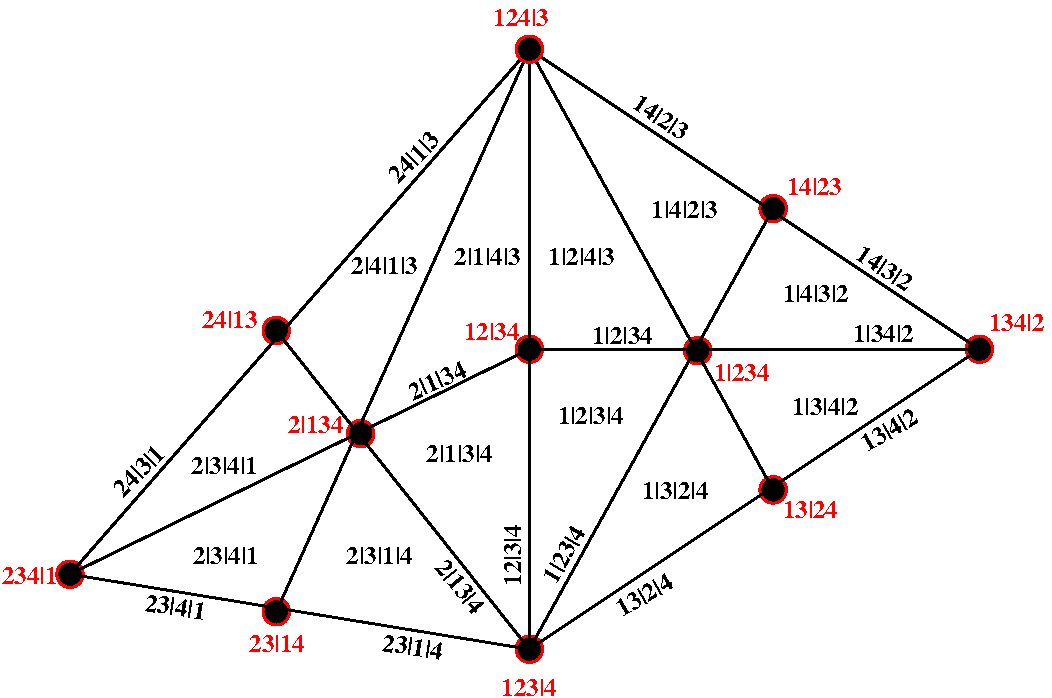
\includegraphics[height=2.5in]{Cox.pdf}
\caption{Two front faces of the Coxeter complex of type A labeled by ordered set partitions.}
\end{figure}


%**Figure of Coxeter complex labeled with ordered set partitions.**

\subsection{Noncommuting Variables}


%% NCSym are symmetric functions indexed by set partitions.  NCQSym are
%% quasisymmetric functions indexed by ordered set partitions, sometimes
%% called set compositions.  (Think of this as analogous to moving from
%% partitions to compositions when one moves from symmetric functions to
%% quasisymmetric functions).


Let $\{x_1, x_2, \ldots \}$ be a collection of non-commuting
variables.  Given $a \in \mathbb{N}^n$, let $\Delta(a)$
be the ordered set partition $(\Delta_1 | \Delta_2 | \ldots | \Delta_k)$ such that 
%flag of subsets $\empty = F_0 \subset F_1 \subset \ldots
%\F_{k+1} =[n]$ such that 
$a$ is constant on each set $\Delta_i$
%\backslash F_{i-1}$ 
and satisfies $a|_{\Delta_i} < a|_{\Delta_{i+1}}$ for all $1 \leq i \leq k$. 
%We call $\mathcal{F}(\omega)$ the flag of $\omega$ and
Define the weight class of $a$ to be the set of vectors $b$
such that $\Delta(b) = \Delta(a)$.  
%The weight class of $a$ consists of all 
%points such that the relative size of their components is the same.  If $a$ is contained in the relative interior of the face $F$ of the Coxeter complex, then the weight class of $a$ consists of all integer points in the relative interior of $F$.

\begin{example}
For $a = (3,2,2,3,1) \in \mathbb{N}^5$, $\Delta(a) =
(5|23|14)$.  The weight class of $a$ consists of all vectors $x
\in \mathbb{N}^5$ such that $x_5 < x_2 = x_3 < x_1 = x_4$. 
\end{example}


The weight class specifies the relative ordering of coordinates and a
weight class is simply all points in the relative interior of a cone
of the Braid arrangement and hence naturally associated to (the relative interior) of a face of
the Coxeter complex.  A satisfiable Scheduling problem corresponds to a union of these open faces.   


\begin{definition}
A function in non-commuting variables is called quasisymmetric (an element of NCQsym) if
$\forall \, \gamma, \tau \in \mathbb{N}^n$ such that $\gamma$ and $\tau$
are in the same weight class, $\Delta(\gamma) =
\Delta(\tau)$, the coefficient of $x_{\gamma_1}x_{\gamma_2} \cdots
x_{\gamma_n}$ is the same as the coefficient of $x_{\tau_1}x_{\tau_2} \cdots x_{\tau_n}$.
\end{definition}

Let $\Phi$ be an ordered set partition.  Define the monomial quasisymmetric function in non-commuting variables indexed by $\Phi$ as follows:
$$\ncM_{\Phi} = \sum_{a \in \mathbb{N}^n \, \Delta(a) = \Phi} {\bf{x}}_{a}$$

Alternatively, quasisymmetric functions in non-commuting variables can be defined as any function which can be expressed as a sum of monomial terms $\ncM_{\Phi}$

%% Again, one could alternatively define the quasisymmetric functions in
%% non-commuting variables to be any sum of the monomials.  Most of the
%% algebra of NCQSym is done at the level of monomials or other bases
%% indexed by ordered set partitions without reference to the specific
%% variables.  


\begin{example}

Consider the weight class of  points that satisfy $a_1 = a_3 < a_2 = a_4$.  The corresponding ordered set partition $\Psi$ is $(13|24)$.  
$$M_{\Psi} = x_1x_2x_1x_2 + x_1x_3x_1x_3 + x_2x_3x_2x_3 + x_3x_4x_3x_4 + \cdots$$  

\end{example}


Informally, an nc-quasisymmetric function corresponds to a
$k$-schedule where $k$ has been taken to infinity, i.e. there is no
deadline.  Recall the example above on two jobs such that job 2 must
start after job 1 unless they start at the same time.  This
corresponds to the weight classes $\{x_1 < x_2, x_1 = x_2\}$ and the
nc-quasisymmetric function $\ncM_{1|2} + \ncM_{12}$.  In order to
impose a deadline, or $k$ time slots, we will restrict to a
polynomial.


\begin{figure}[h]
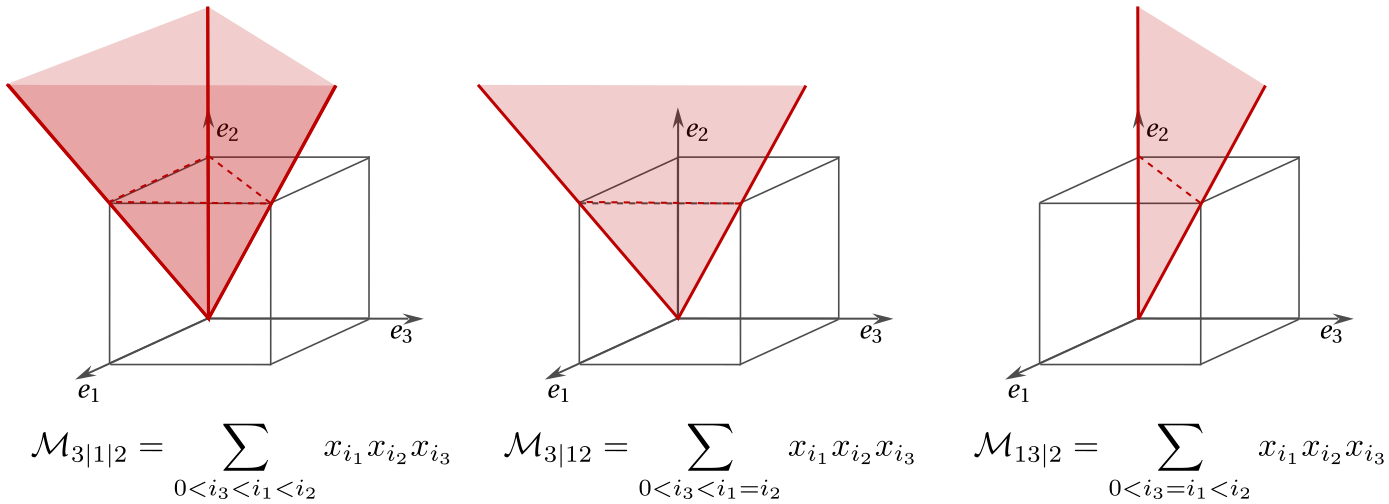
\includegraphics[angle=270,width=14cm]{cone}
\caption{\label{fig:cone}Correspondence between monomial ncquasisymmetric functions and simplicial unimodular cones in the braid arrangement.}
\end{figure}


%job 1 is started immediately in which case they may both start at the same time.  


\subsection{From NCQsym to QSym to Polynomials}
Although not strictly necessary to arrive at a polynomial, we will also be interested in the intermediate specialization to a quasisymmetric function.  


As we have seen, elements of QSym are naturally indexed by
compositions and elements of NCQSym are naturally indexed by ordered
set partitions.  
One way to map from NCQSym back to Qsym is via the type map, which sends ordered set partitions to compositions.
 %We can use the type map from partitions to
%compositions to specialize an element of NCQSym to an element of QSym.
The type map of a partition simply records the size of each block.
$$\textrm{type}(B_1|B_2|\cdots|B_n) = (|B_1|, |B_2|, \cdots, |B_n|)$$
If $\mathcal{S} \in NCQSym$ is written as a sum of monomial terms,
applying the type map to each index is equivalent to allowing the
variables to commute.

\begin{example}
Let $$\mathcal{S} = \ncM_{1|23} + \ncM_{3|21} + \ncM_{2|1|3}$$ be an element of NCQSym written in terms of monomials.  Then 
\begin{align*}
\textrm{type}(\mathcal{S}) & =  M_{\textrm{type} (1|23)} + M_{\textrm{type} (3|12)} + M_{\textrm{type} (2|1|3)} \\
&  = 2 M_{(1,2)} + M_{(1,1,1)}.
\end{align*}
 Where the last line is a quasisymmetric function given in the monomial basis indexed by compositions.  
\end{example}

%\begin{remark}  There are other natural ways to map from ordered set partitions to compositions as we will see.  In particular, if the ordered set paritions correspond to fl


Given a quasisymmetric function in non-commuting variables (or
commuting), there is a naturally associated polynomial function
defined by setting the first $k$ variables equal to $1$.  For a scheduling problem, this polynomial counts the number of $k$-schedules.  

\begin{example}
Writing ${\bf 1}^k$ for the vector of $1$s of length $k$, and continuing the example above, we have 
$$ \mathcal{S}({\bf 1}^k) = 2 {k \choose 2} + {k \choose 3}.$$  
\end{example}

In general, the schedule counting polynomial $\xi_S(k)$ is defined as
\[
  \xi_S(k) = \# \text{$k$-schedules $\omega$ such that $\phi(\omega)$ is true}.
\]

In summary, we have the following lemma.

\begin{lemma}
If $S$ is a scheduling problem on $n$ items, then $\SSS_S$ is an ncquasisymmetric function and $\xi_S$ is a polynomial of degree at most $n$. Moreover, $\SSS_S$ specializes to $\xi_S(k)$ when we substitute $1$ for $k$ different variables in $\SSS_S$ and $0$ for all others, i.e.,
\[
  \SSS_S({\bf 1}^k) = \xi_S(k).
\]
Note that the result of this specialization is independent of which variables are set to 1.
\end{lemma}

\comment{fb: We should add a statement about quasisymmetric functions to this lemma.}

\subsection{The Fundamental Basis}

The scheduling function $\SSS_S$ is a quasisymmetric function in
non-commuting variables and $\xi_S(k)$ is a polynomial.  The structure
of $\Sigma(S)$ also yields information on the the intermediate
quasisymmetric function $QS_S$.

  If $\SSS_S$ is given in the monomial
bases indexed by ordered set partitions, $QS_S$ is defined as the
quasisymmetric function formed by applying the type map to each
monomial term.  We will be interested in the expansion of $QS_S$ in
bases other than the monomial, in particular the fundamental basis.
To this end we review analogous bases in NCQSym which allow us to also
specialize via the type map.

Recall that the fundamental quasisymmetric functions are defined from the monomial quasisymmetric functions as follows.  For any composition $\alpha$, 
$$L_{\alpha} := \sum_{\beta:\beta \textrm{ refines } \alpha} M_{\beta}.$$
The poset of all compositions that refine $\alpha$, ordered by the refinement relation, forms a boolean lattice of dimension $n-i$ where $n$ is the total number of elements in the ground set and $i$ is the length of $\alpha$. For example, the composition $3+1$ is refined by $1+2+1$, $2+1+1$ and $1+1+1+1$, where $1+2+1$ and $2+1+1$ are incomparable under the refinement relation.

In the case of nc-quasisymmetric functions, we can perform a similar construction as follows. Let $\Phi_\text{coarse}$ and $\Phi_\text{fine}$ and be two ordered set partitions such that $\Phi_\text{fine}$ is a permutation\footnote{$\Phi_text{fine}$ is an ordered set partition of length $n$, i.e., a maximum of the refinement relation.} that refines $\Phi_\text{coarse}$. Then the poset of all ordered set partitions $\Phi$ in between $\Phi_\text{coarse}$ and $\Phi_\text{fine}$ under the refinement relation forms again a boolean lattice of dimension $n-i$ where $i$ is the length of $\Phi_\text{coarse}$. Moreover, the type map gives an isomorphism from this boolean lattice to the boolean lattice of all compositions refining $\operatorname{type}(\Phi_\text{coarse})$. Thus, when we define
\[
  \ncL_{(\Phi_\text{coarse};\Phi_\text{fine})} = \sum_{\Phi_\text{coarse}\leq \Phi \leq \Phi_\text{fine}} \ncM_\Phi
\]
we obtain an nc-quasisymmetric function $\ncL_{(\Phi_\text{coarse};\Phi_\text{fine})}$ that specializes to $L_{\operatorname{type}(\Phi_\text{coarse})}$ when we allow variables to commute.

As $(\Phi_\text{coarse};\Phi_\text{fine})$ ranges over all such pairs of ordered set partitions, which are comparable under the refinement relation and  where$\Phi_\text{fine}$ has length $n$, the functions $\ncL_{(\Phi_\text{coarse};\Phi_\text{fine})}$ form a generating system of the linear space of all nc-quasisymmetric functions. However, they do not form a basis as there are multiple representations of the same quasisymmetric function, for example
\[
  \ncL_{(1|2|3;1|2|3)} + \ncL_{(1|23;1|3|2)} =   \ncL_{(1|23;1|2|3)} +  \ncL_{(1|3|2;1|3|2)}.
\]
We call this the \emph{fundamental generating system} of the nc-quasisymmetric functions. To obtain a basis, we can fix a canonical choice for $\Phi_\text{fine}$ given $\Phi_\text{coarse}$: For any ordered set partition $\Phi$, let $\hat{\Phi}$ denote the permutation refining $\Phi$ with the property that the elements of each part of $\Phi$ are listed in order. For example, if $\Phi=35|247|16$ then $\hat{\Phi}=3|5|2|4|7|1|6$. We then define $L_\Phi:=L_{(\Phi;\hat{\Phi})}$. As $\Phi$ ranges over all ordered set partitions, the functions $L_\Phi$ form a basis for the space of nc-quasisymmetric functions, which we call the \emph{fundamental basis}.

Alternatively, this fundamental basis for nc-quasisymmetric functions can be defined in terms of a \emph{directed refinement relation} $\preceq$ on ordered set partitions given by $\Phi \gtrdot (\Phi_i, \ldots,\Phi_{i-1}, \Phi_i \cup \Phi_{i+1}, \Phi_{i+2}, \ldots \Phi_k)$ where every element of the $i$th block is less than every element of the $i+1$th block. (Note that this order is opposite to the order $\leq_*$ defined in [cite: Zab].(** Draw poset?**)) Then, the $\mathcal{L}$ basis for NCQSym can be defined by
$$\mathcal{L}_{\Phi} := \sum_{\Gamma:\Gamma \preceq \Phi} \ncM_{\Phi},$$
where $\Phi$ ranges over all ordered set partitions. Note this definition coincides with the previous one. Applying the type map to the $\ncL$ basis gives the corresponding quasisymmetric function in the $L$ basis, in such a way that directed refinement on the level of nc-quasisymmetric functions corresponds to refinement on the level of quasisymmetric functions.

\begin{diagram}
NCQSym \ncM & \rTo^{\text{ directed refinement }} & NCQSym \ncL\\
\dTo^{ \text{type}} & & \dTo_{ \text{type}}\\
QSym M & \rTo^{\text{refinement}} & QSym L
\end{diagram}

\begin{example}

Consider the nc-quasisymmetric function 
\begin{align*}
 \SSS & = \ncM_{12|3} + \ncM_{1|23} + \ncM_{1|2|3} + \ncM_{2|1|3} + \ncM_{1|3|2}\\
      & = \ncL_{12|3} + \ncL_{1|23} - \ncL_{1|2|3} + \ncL_{2|1|3} + \ncL_{1|3|2}.
\end{align*}

\begin{align*}
 QS & = M_{(2,1)} + M_{(1,2)} + 3M_{(1,1,1)}\\
 & = L_{(2,1)} + L_{(1,2)} + L_{(1,1,1)}\\
& = L_{\textrm{type}(12|3)} + L_{\textrm{type}(1|23)} - L_{\textrm{type}(1|2|3)} + L_{\textrm{type}(2|1|3)} + L_{\textrm{type}(1|3|2)}.
\end{align*}

\end{example}


Clearly $\ncL$ positivity of a nc-quasisymmetric function gives a sufficient although not neccesary condition for  $L$ positivity of the quasisymmetric specialization. 


%% \begin{remark}
%% (** Do we want this remark? **) Although one could define a partial order on ordered set partitions
%% simply by refinement, and sum over all refinements, such elements would not fit into our diagram above.  Consider the example above, ...
%% \end{remark}



%% \begin{itemize}
%% \item Give an example that at the level of ordered set partitions,
%% you can not simple sum over refinements and then take the type map.

%% \item Define partial ordering, basis and co-basis as in Zabrocki.

%% \item Draw diagram with type maps.

%% \item Note that positivity in NCL is sufficient although not necessary for positivity in L.
%% \end{itemize}

\begin{theorem} \label{unique} Let $S$ be a scheduling problem on $d$ items.  If the forbidden configuration $\Sigma(S)$ is a subcomplex of the Coxeter complex and if for each total ordering of $[d]$ there is a unique coarsest schedule satisfying $S$, then $\SSS_S$ is $\ncL$-positive and therefore $QS$ is $L$-positive. 
\end{theorem}


\begin{proposition}
Scheduling problems of the form of Theorem~\ref{posets} satisfy the conditions of Theorem~\ref{unique} and are hence $\ncL$-positive.
\end{proposition}

\begin{proof}
Discuss how each $C_{i,j}$ defines a poset of regions in the Coxeter complex and how this yields coarsest.
\end{proof}

\begin{example}
Returning to the chromatic scheduling problem, Theorem~\ref{Hilbert}
was shown by Steingrimmson in [cite], that $\Sigma(S)$ had a convex
ear decomposition by Hersch and Swartz [cite], and L-positivity of the
chromatic symmetric function by [cite].  The chromatic scheduling
problem can also be seen to satisfy the conditions of
Theorem~\ref{posets} and hence Therorem~\ref{unique}.  This was shown
in [cite GP] by considering a larger class of scheduling problems
defined for generalized permutahedron.  

The scheduling problem of [GP] is defined by taking, for each vertex
$v$ of a generalized permutahedron $P$, the conjugation of all
hyperplanes defining $v$.  Hence the valid $\omega$ schedules
correspond to all integer points in the interior of the normal fan or
equivalently the forbidden configuration is the entire co-dimension
one skeleton $P$.  The normal fans of generalized permutahedron are
refined by the Braid arrangement and the $C_{i,j}$ of
Theorem~\ref{posets} correspond to all interiors of the maximal cones.
In cite[GP], the conditions of Theorem~\ref{unique} are established in
the Hopf monoid setting of directed faces.  The chromatic scheduling
problem is the special instance of the generalized permutahedron
scheduling problem for graphical zonotopes.  As another special
instance, the quasisymmetric function $QS$ for matroid polytopes is
the Biller-Jia-Reiner quasisymmetric function for matroids.
\end{example}


Scheduling problems satisfying the form of Theorem~\ref{posets} can be
described in terms of $P$-partitions for posets $P$ with all strict
edges.  Again, each $C_{i,j}$ is a collection of strict edges of the
form $x_a < x_b$ which defines a poset.  The quasisymmetric function
$QS$ restricted to a single $C_{i,j}$ is the generating function
$K_{(P,\omega)}$ where $\omega$ is a ``fully un-natural'' labelling of
$P$.  For schedules with a single $C_{i,j}$, Theorem~\ref{unique}
gives the Fundamental theorem of quasisymmetric functions, i.e. the
expansion of $K_{(P,\omega)}$ in the fundamental basis by descent
sets.  In this case, with all strict labels, the unique coarsest
elements for each ordering are also defined by the descent sets.


Theorem~\ref{unique} is neither strictly stronger nor weaker than the
$K_{(P,\omega)}$ expansion.  Posets with non-strict edges may easily
be non-positive in the $\ncL$ basis and many scheduling problems
satisfy the conditions of Theorem~\ref{unique} but do not arise from
any poset or P-partition structure.

\begin{example} 
Consider the scheduling nc-quasisymmetric function,

\begin{align*}
\SSS_S & = \ncL_{24|13} + \ncL_{4|2|13} + \ncL_{24|3|1} + \ncL_{2|14|3} + \ncL_{2|1|34} + \ncL_{4|2|3|1}\\
& = \ncM_{24|13} + \ncM_{2|4|13} + \ncM_{24|1|3} + \ncM_{2|4|1|3} + \ncM_{4|2|13} + \ncM_{4|2|1|3} + \ncM_{24|3|1}\\
& + \ncM_{2|4|3|1} + \ncM_{2|14|3} + \ncM_{2|1|4|3} + \ncM_{2|1|34} + \ncM_{2|1|3|4} + \ncM_{4|2|3|1}.
\end{align*}

This scheduling problem does satisfy the conditions of Theorem~\ref{unique}, but it does not satisfy the conditions of Theorem~\ref{posets}.  In particular, the collection of valid schedules forms a non-convex collection of Braid cones.

\end{example}


%
%Some ``bigger picture'' thoughts about quasisymmetric functions and a few classes thought about together. 

%Consider the following quasisymmetric functions:

%% \begin{itemize}
%% \item QGP: (Quasi Generalized Permutahedron) - this includes Stanley chromatic quasisymmetric function for graphs and the Biller-Jia-Reiner quasisymmetric functions for matroids as special cases.

%% In terms of ordered set partitions, these are all integer points in the interiors of all maximal cones of the fan.  In terms of the forbidden subcomplex, we are getting rid of all codimension one faces.  

%% \item QBergman: This is defined for any matroid, over the matroid polytope.

%% \item QEhrenborg: Not really it's name, but Richard defined a class of quasisymmetric functions for posets.

%% \end{itemize}


\section{Scheduling Problems}
\label{sec:scheduling-problems}

\subsection{The monomial basis and the Ehrhart $f^*$-vector}

For an ordered set partition $\Phi=(\Phi_1,\ldots,\Phi_m)$, we define the relatively open cone $\cone(\Phi)\subset\RR^n$ to be the set of all $a\in\RR^n$ that satisfy the constraints
\begin{eqnarray*}
0 < a_i && \text{for all $i\in[n]$}, \\
a_i = a_j && \text{for all $l\in[m]$ and $i,j\in\Phi_l$}, \\
a_i < a_j && \text{for all $l_1 < l_2\in[m]$ and all $i\in\Phi_{l_1}, j\in\Phi_{l_2}$}.
\end{eqnarray*}
Equivalently, $\cone(\Phi)$ is the set of all real vectors $a$ in the positive orthand, $\RR_{> 0}^n$ such that $\Delta(a)=\Phi$. 
\[
\cone(\Phi) = \mset{a\in\RR_{> 0}^n}{\Delta(a)=\Phi}.
\]
The cones $\cone(\Phi)$ are simplicial. If $\Phi$ ranges over all ordered set partitions of $[n]$, these cones form a triangulation $T^n$ of the positive orthand $\RR_{> 0}^n$, in particular,
\[
  \RR_{> 0}^n = \bigcup_\Phi \cone(\Phi),
\]
where the union is disjoint. Thus, a cone $\cone(\Phi')$ is a face of the cone $\cone(\Phi)$ if and only if $\Phi'$ is a coarsening of $\Phi$, or equivalently, $\Phi$ is a refinement of $\Phi'$. Note that the complex $\{\cone(\Phi) \;|\; \Phi\}$ is a partial simplicial complex, as the faces with $x_i=0$ for some $i$ are missing.

This triangulation of $\RR_{> 0}^n$ can also be obtained by subdividing the positive orthand according to the Braid arrangement of all hyperplanes $x_i=x_j$. Combinatorially, the resulting partial polyhedral complex is equivalent to a cone over the Coxeter complex of type $A$. 

As mentioned in the introduction, we can associate to every $a\in\NN^n$ a monomial in non-commuting variables $x_{a_1}\cdot\ldots\cdot x_{a_n}$ which we abbreviate as $x_a$. In this way, we can associate to every set $A\subset\NN^n$ of lattice points a formal sum $N(A)$ of monomials in non-commuting variables
\[
  N(A) = \sum_{a\in A} x_a.
\]

The function $N$ maps the cones $\cone(\Phi)$ to the monomial ncquasisymmetric functions $\ncM_\Phi$, more precisely,
\[
  N(\cone(\Phi)\cap\ZZ^n) = \ncM_\Phi.
\]
Conversely, we can think of any ncquasisymmetric function $\SSS$ with non-negative coefficients in the monomial basis as a multiset of cones in the positive orthand, where the multiplicity of lattice points in $\cone(\Phi)$ is given by the coefficient of $\ncM_\Phi$ in $\SSS$. In the case of scheduling ncquasisymmetric functions we can conclude that for any scheduling problem $S$, the ncquasisymmetric function $\SSS_S$ has coefficients $0$ or $1$ in the monomial basis.

Substituting 1s for variables $x_1,\ldots,x_k$ and 0s for variables $x_{k+1},\ldots$ effectively sets all monomials $x_a$ to $1$ for which $a_i \leq k$ for all $i$, and it sets all monomials $x_a$ to $0$ for which $a_i > k$ for some $i$. Thus substituting ${\bf 1}^k$ into $\ncM_\Phi$ corresponds to taking the intersection of the cone $\cone(\Phi)$ with the open cube $(0,k+1)^n$, i.e.,
\[
 N(\cone(\Phi)\cap(0,k+1)^n\cap\ZZ^n) = \ncM_\Phi({\bf 1}^k) =  \xi_\Phi(k). 
\]
We observe that
\[
  \cone(\Phi)\cap(0,k+1)^n = (k+1)\cdot (\cone(\Phi)\cap(0,1)^n), 
\]
since the hyperplanes defining $\cone(\Phi)$ all go through the origin. We have thus found that
\begin{eqnarray}
\label{eqn:spec ncM}
  \ncM_\Phi({\bf 1}^k) = \xi_\Phi(k) = \ehr_{\cone(\Phi)\cap(0,1)^n}(k+1),
\end{eqnarray}
that is, $\ncM_\Phi({\bf 1}^k)$ is the Ehrhart polynomial of the open polytope $\cone(\Phi)\cap(0,1)^n$, up to a shift of 1. As we will see below, $\cone(\Phi)\cap(0,1)^n$ is a relatively open unimodular simplex of dimension $m$, whence
\[
  \xi_\Phi(k) = \binom{k}{m}.
\]

Let $S$ be a scheduling problem on $n$ items. For any vector $a\in\RR^n_{> 0}$ we write $S(a)$ to denote the boolean value of whether or not $a$ satisfies the constraints imposed by $S$. Note that $S(a)$ depends only on the relative order of the component $a_i$, and therefore is entirely determined by the ordered set partition $\Phi=\Delta(a)$. We use $S(\Phi)$ to denote the boolean value of whether or not $S(a)$ is satisfied for any (or, equivalently, all) $a$ with $\Delta(a)=\Phi$. Geometrically, this means that $S$, viewed as a function on $\RR^n_{>0}$, is constant on each of the open cones $\cone(\Phi)$, i.e., on the relative interior of, each face of the above triangulation $T^n$ of $\RR^n_{> 0}$.

These observations lead to the following theorem about the coefficients of $\SSS_S$ in the monomial basis and the coefficients of $\xi_S$ in the binomial basis $\binom{k}{i}$ for $i=0,\ldots,n$.

\begin{theorem}
Let $S$ be a scheduling problem on $n$ items. Then $\SSS_S$ is an nc-quasisymmetric function of the form
\[
  \SSS_S = \sum_{\Phi:S(\Phi)} \ncM_\Phi
\]
where the sum ranges over all ordered set partition $\Phi$ that satisfy $S$. In particular, the coefficients of $\SSS_S$ in the monomial basis are either 0 or 1.

Moreover, $\xi_S$ is a polynomial of degree at most $n$. The coefficients $f_1,\ldots,f_n$ of $\xi_S$, given by
\[
  \xi_S(k) = \sum_{i=1}^n f_i\binom{k}{i}
\]
or, equivalently,
%\[
%  z^{-1}\sum_{k\geq 1} \ehr_S(k)z^k = z^{-1}(\frac{f_0z^1}{(1-z)^1} + \cdots + \frac{f_dz^{d+1}}{(1-z)^{d+1}})
%  z^{-1}\sum_{k\geq 0} \ehr_S(k+1)z^{k+1} = ...
%  \sum_{k\geq 0} \ehr_S(k+1)z^k = ...
%\]
\[
  \sum_{k\geq 0} \xi_S(k)z^k = \frac{f_1z^1}{(1-z)^2} + \cdots + \frac{f_nz^{n}}{(1-z)^{n+1}},
\]
satisfy the following properties:
\begin{enumerate}
\item $f_i\in\ZZ$,
\item $0\leq f_i \leq i!\cdot S(n,i)$,
\item $f_i$ counts the number of ordered set partitions $\Phi$ of $[n]$ into $i$ non-empty parts such that $S(\Phi)$ holds.
\end{enumerate}
\end{theorem}

\begin{proof}
Let $S$ be a scheduling problem. Let $A$ denote the set of all vectors $a\in\RR^n_{> 0}$ such that $S(a)$ holds true. Then, from the above observations, we obtain
\[
 \SSS_S = \sum_{a\in A\cap\ZZ^n} x_a = \sum_{\Phi:S(\Phi)} \ncM_\Phi,
\]
where the latter sum ranges over all ordered set partitions $\Phi$ for which $S(\Phi)$ holds true. This means in particular that the coefficients of $\SSS_S$ in the monomial basis are either 1 or 0, indicating which open cones $\cone(\Phi)$ are contained in $A$ and which are disjoint from $A$.

Let $\Phi$ be an ordered set partition with $n$ non-empty parts, i.e., a permutation of the numbers $1,\ldots,n$. Assume without loss of generality that $\Phi=1|2|\cdots|n$. Then
\[
  \cone(\Phi)\cap [0,1]^n = \mset{a\in[0,1]^n}{a_1<a_2<\ldots<a_n}
\]
which is easily seen to be a unimodular simplex with vertices $(0,\ldots,0)$, $(0,\ldots,0,1)$, $(0,\ldots,0,1,1)$, $\ldots$, $(1,\ldots,1)$. If, more generally, $\Phi=(\Phi_1,\ldots,\Phi_i)$ is any ordered partition with $i\in[n]$ non-empty parts, then $\cone(\Phi)\cap[0,1]^n$ is an $i$-dimensional unimodular simplex with vertices $v_0,\ldots,v_i$ where $v_j$ for $j=0,\ldots,i$ has entries 
\[
 v_{j,k} = \choice{1 & \text{if }k\in\Phi_{i-l} \text{ for some } 0\leq l < j, \\ 0 & \text{otherwise.} }
\]
In particular, $v_0= \mathbf{0}$ and $v_i=\mathbf{1}$. 

Passing to the open cube, we find that the collection of relatively open simplices $\cone(\Phi)\cap (0,1)^n$ where $\Phi$ ranges over the ordered set partitions of $[n]$ is a partial simplicial complex that triangulates the open cube $(0,1)^n$. If $\Phi$ has $i$ parts, then $\cone(\Phi)\cap (0,1)^n$ is a relatively open $i$-dimensional simplex whose Ehrhart polynomial is
\[
  \ehr_{\cone(\Phi)\cap (0,1)^n}(k) = \binom{k-1}{i} = \#\cone(\Phi)\cap (0,k)^n \cap \ZZ^n
\] 

It follows that
\begin{eqnarray*}
  \xi_S(k) &=& \#A\cap(0,k+1)^n\cap\ZZ^n \\
  &=& \ehr_{A\cap(0,1)^n}(k+1) \\
  &=& \sum_{\Phi:S(\Phi)} \ehr_{\cone(\Phi)\cap(0,1)^n}(k+1) \\
  &=& \sum_{i=1}^n f_i\binom{k}{i}
\end{eqnarray*}
where $f_i$ is the number of ordered set partitions $\Phi$ with $i$ non-empty parts. Note that the binomial coefficients $\binom{k}{i}$ for $i=0,\ldots,n$ form a basis of the space of polynomials of degree at most $n$, to that the coefficients $f_i$ are determined by the polynomial $\xi_S(k)$. To see that the above generating function definition of the coefficients $f_i$ is equivalent, note that 
\[
  \frac{1}{(1-z)^{d+1}} = \sum_{k\geq 0} \binom{k+d}{d} z^k
\]
from which we get the desired identity by algebraic manipulation.

From this counting interpretation of the coefficients $f_i$ it follows immediately that the $f_i$ are non-negative integers. Moreover there are at most at most $i!\cdot S(n,i)$ ordered set partitions of $[n]$ with $i$ non-empty parts \cite{something}, which proves the upper bound on the $f_i$. \comment{Todo: check upper bound formula and find reference: OEIS.}

Finally, the fact that $\SSS_S$ specializes to $\xi_S(k)$ follows immediately from the specialization (\ref{eqn:spec ncM}).
\end{proof}

\subsection{Triangulations and their Allowed and Forbidden Subcomplexes}

The Braid arrangement, consisting of all hyperplanes
\[
  H_{i,j} = \mset{a\in\RR^n}{a_i \leq a_j}
\]
for $1\leq i,j\leq n$, induces subdivisions $\TRn$, $\TP$, $\TC$, and $\TS$ of the space $\RR^n$, the positive orthand $\RR^n_{> 0}$, the open unit cube $(0,1)^n$ and the $n-2$ dimensional sphere
\[
S^{n-2}=\mset{x\in\RR^n}{||x||_2 = 1, \sum_{i=1}^n = 0},
\]
respectively. The faces of these subdivisions are the regions of the respective ground set where the function $\Delta$, mapping points $a\in\RR^n$ to ordered set partitions $\Phi$, is constant. The faces of $\TRn$ are relatively open polyhedral cones, each containing the lineality space $\mset{a\in\RR^n}{a_i=a_j \; \forall i,j}$. The faces of $\TP$ are pointed, relatively open simplicial cones. The faces of $\TC$ are relatively open unimodular simplices. The faces of $\TS$ are sections of the $n-2$ sphere. Combinatorially, however, $\TS$ is equivalent to a simplicial complex known as the Coxeter complex of type $A_{n-1}$ \cite{something}.

All of these complexes are closely related. In fact, $\TRn$, $\TP$, and $\TC$ are all combinatorially equivalent, as the function $\Delta$ defines a bijection between their sets of faces that preserves incidences. In particular, the faces of these three complexes are in one-to-one correspondence with the ordered set partions $\Phi$ of $[n]$ into non-empty parts. The only difference with $\TS$ is that there is no face of $\TS$ corresponding to the partition with only one part. Combinatorially, the other complexes are the cone over $\TS$. As these geometric objects are so closely related, we will frequently draw no clear distinction between them and refer loosely to the triangulation $\Tn$. It will be clear from context which of these objects we are referring to in each case.

We write $\sigma\in\Tn$ to denote that $\sigma$ is a face of the triangulation $\Tn$. We use $\sigma_\Phi$ to mean the face of $\Tn$ corresponding to the ordered set partition $\Phi$. A scheduling problem $S$ defines which faces of in these complexes are allowed and which are forbidden. Recall that $S(\Phi)$ denotes the truth value of whether $S(a)$ holds for any (or, equivalently, all) $a\in\RR^n$ with $\Delta(a)=\Phi$. We define the \emph{allowed subcomplex} $\allow(S)$ of the triangulation $\Tn$ to be the set of faces 
\[
  \allow(S) = \mset{\sigma_\Phi \in \Tn}{S(\Phi)}.
\]
Correspondingly, define the \emph{forbidden subcomplex} $\forb(S)$ to be the set of faces
\[
  \forb(S) = \mset{\sigma_\Phi \in \Tn}{\neg S(\Phi)}.
\]

\comment{TODO: Check if this example needs to be rewritten to improve the flow.}

\begin{example} As remarked above, a particularly familiar scheduling polynomial is the chromatic polynomial of a graph.  In this case, the scheduling problem simply specifies which variables can not be equal to each other, $x_i \neq x_j$ for $\{i,j\}$ an edge of the graph. $\xi_S$ is the chromatic polynomial.  The quasisymmetric function obtained by taking the type map on $\SSS_S$ is Stanley's chromatic symmetric function (the quasisymmetric function happens to be fully symmetric in this case).  Gebhard and Sagan studied (essentially) $\SSS_S$ as a symmetric function in non-commuting variables.  Steingrimmson's coloring complex is 
%the collection of ordered set partitions which require at least one edge in at least one block, namely 
the forbidden configuration of the scheduling problem.  
Much work has been done to understand the coloring complex in order to better understand the chromatic polynomial.  This avenue is possible because the Hilbert series connection as shown in [cite:Ein].
\end{example}

Clearly, $\allow(\neg S)=\forb(S)$. This notion of complementarity translates into basic observations about the counting function defined by $S$. Let 
\[
  \SSS_{\top^n} = \sum_{a\in\NN^n} x_a
\]
denote the nc-quasisymmetric function corresponding to all lattice points in the positive orthand. Furthermore, note that $(k-1)^n$ is the Ehrhart polynomial of the open cube $(0,k+1)^n$. Then we have the following complementarity result.

\begin{lemma}
Let $S$ be a scheduling problem on $n$ items given by the boolean formula $\phi$. Let $\neg S$ denote the scheduling problem given by $\neg\phi$. Then 
\begin{eqnarray*}
  \xi_{S}(k) + \xi_{\neg S}(k) &=& (k-1)^n, \\
  \SSS_S + \SSS_{\neg S} &=& \SSS_{\top^n}.
\end{eqnarray*}
\end{lemma}

Note that passing from $\SSS_S$ to $\SSS_{\neg S}$ swaps coefficients 0 and 1 in the monomial basis. Also passing from $\xi_S$ to $\xi_{\neq S}$ replaces the coefficient $f_i$ with $i!\cdot S(n,i) - f_i$, thus interchanging the roles of the upper and lower bound on the $f_i$ in the theorem.

\begin{proof}
The result on $\SSS_S$ is immediate from the above observations. For the result on $\xi_S$, note that 
\[
 \xi_{S}(k) + \xi_{\neg S}(k) = \ehr_{A\cap(0,1)^n}(k+1) +  \ehr_{(0,1)^n\setminus A}(k+1) = \ehr_{(0,1)^n}(k+1) = (k-1)^n.
\]
\end{proof}

\subsection{The fundamental basis and the $h$-vector}

We have seen how we can use the $f$-vectors of the allowed and forbidden complexes of a scheduling problem $S$, that is the number of faces of various dimension, to obtain constraints on the counting functions, in particular the scheduling polynomial $\xi_S$. Geometrically, this corresponds to decomposing $\allow(S)$ as a disjoint union of relatively open unimodular simplices of different dimension. However, there are other important ways of decomposing simplicial complexes. The idea of writing a simplicial complex as a disjoint union of half-open simplices gives rise to the notion of an $h$-vector.

We have seen in the preliminaries that the Ehrhart polynomial of a $d$-dimensional unimodular simplex $\Delta^d_i$ with $i$ open faces is
\[
  \ehr_{\Delta^d_i}(k) = \binom{k+d-i}{d}.
\]
A $d$-dimensional simplex can have between 0 and $d+1$ open faces, and indeed it turns out that the polynomials $\binom{k+d-i}{d}$ for $i=0,\ldots,d+1$ generate the space of all polynomials of degree at most $d$. That is, for every polynomial $p$ of degree at most $d$ there exist coefficients $h_0,\ldots,h_{d+1}$ such that
\[
  p(k) = \sum_{i=0}^{d+1} h_i \binom{k+d-i}{d}.
\] 
However, these coefficients $h_i$ are not uniquely determined as there is one degree of freedom too many. There are two different conventions for normalization, which determine the coefficient vector uniquely. The first convention is to fix $h_0=1$, which gives rise to the $h$-vector as commonly used in the study of simplicial complexes \cite{something}. This choice is motivated by the notion of a shelling, which induces a partition of a triangulation into half-open simplices in which exactly one is closed. The second convention is to fix $h_{d+1}=0$, which gives rise to the $h^*$-vector (or Ehrhart $\delta$-vector) used in Ehrhart theory \cite{something}. Geometrically, the $h^*$- and $h^\circ$-vectors correspond to partitions of a triangulation into half-open simplicies without fully-open simplicies. It is important to note, however, that the two coefficient vectors are well-defined, even if such partitions do not exist.

Formally, given numbers $f_0,\ldots,f_d$, the \emph{$h$-vector} $h_0,\ldots,h_{d+1}$ and the \emph{$h^*$-vector} $h^*_0,\ldots,h^*_{d}$ are defined, respectively, via $h_0=1$ and
\begin{eqnarray*}
  \sum_{i=0}^{d} f_i \binom{k-1}{i} & = &
  \binom{k+d}{d} + \sum_{i=1}^{d+1} h_i \binom{k+d-i}{d} 
  \\ 
  & = & \sum_{i=0}^{d} h^*_i \binom{k+d-i}{d} 
\end{eqnarray*}
Generally, the vector $(f_0,\ldots,f_d)$ is going to be the $f$-vector $f(X)$ of a partial simplicial complex $X$, which means that $f_i$ denotes the number of $i$-dimensional faces of $X$. Correspondingly, the $h$- and $h^*$-vectors of $X$ are defined via the above relations, and are denoted by $h(X)$ and $h^*(X)$, respectively. All of these definitions work for partial complexes as well.

Alternatively, instead of defining the $h$- and $h^*$-vectors of $X$ in terms of $f(X)$, it is possible to define them in terms of the Ehrhart polynomial $\ehr_X$ via $\ehr_X(k) = \sum_{i=0}^{d} f_i \binom{k-1}{i}$. Note that if $X$ is a $d$-dimensional partial unimodular integral simplicial complex these two definitions yield the same result. As all simplicial complexes considered in this article are unimodular, we will use both definitions interchangeably. In general, we are going to use $f(p)$, $h(p)$, and $h^*(p)$ to denote the $f$-, $h$- and $h^*$-vectors of a polynomial $p$ determined via $p(k)=\sum_{i=0}^{d} f_i \binom{k-1}{i}$.

On the level of generating functions, the above definitions can be expressed as follows. Let $p(k)=\sum_{i=0}^{d} f_i \binom{k-1}{i}$. Then the $h$- and $h^*$-vectors can be defined, equivalently, by 
\begin{eqnarray*}
1 + \sum_{k=1}^\infty p(k) z^k & = &  \frac{\sum_{i=0}^{d+1}h_i z^i}{(1-z)^{d+1}} \;\;\; \text{ and } \\
\sum_{k=0}^\infty p(k) z^k & = &  \frac{\sum_{i=0}^{d}h^*_i z^i}{(1-z)^{d+1}}, \\
\end{eqnarray*}
respectively. Note that 
\[ 
h^*_0=\sum_{i=0}^d (-1)^i f_i
\]
from which it follows that the $h$- and $h^*$-vectors of a complex $X$ coincide if and only if the Euler characteristic of $X$ is one.

In particular, the scheduling polynomial encodes data about the allowed and forbidden subcomplexes. Regarding the $h$-vector, for example, the following theorem holds. Analogous statements about the $h^*$-vector are straightforward to derive using the same technique.

\begin{theorem}
\label{Hilbert}
Let $S$ be a scheduling problem. Then the $h$-vector of the shifted scheduling polynomial $\xi_S(k-1)$ is the $h$-vector of the allowed subcomplex $\allowC(S)$ and the $h$-vector of the polynomial $(k-2)^n-\xi_S(k-1)$ is the $h$-vector of the forbidden subcomplex $\forbC(S)$, i.e.,
\begin{eqnarray*}
  h(\xi_S(k-1)) &=& h(\allowC(S)),   \text{ and}\\
  h((k-2)^n - \xi_S(k-1)) &=& h(\forbC(S)),
\end{eqnarray*}
or equivalently,
\begin{eqnarray*}
 1 + z\sum_{k = 0}^\infty \xi_S(k) z^k &=& \frac{\sum_{i=0}^{d+1} h_i(\allow(S)) z^i}{(1-z)^{d+1}}, \text{ and} \\
 1 + z\sum_{k = 0}^\infty \left( (k-1)^n - \xi_S(k) \right) z^k &=& \frac{\sum_{i=0}^{d+1} h_i(\forb(S)) z^i}{(1-z)^{d+1}}.
\end{eqnarray*}
\end{theorem}

\comment{TODO: Credit work with Marcelo here.}

\begin{proof}
Let $S$ be a scheduling problem. As we have seen in the previous two sections, we have
\[
  \xi_S(k) = \ehr_{\allow(S)}(k+1) \;\;\; \text{ and } \;\;\; (k-1)^n - \xi_{S}(k) = \ehr_{\forb(S)}(k+1),
\]
where we are working with the allowed and forbidden partial subcomplexes of the open cube $(0,1)^n$. The partial complexes $\allowC(S)$ and $\forbC(S)$ are partial subcomplexes of $\TC$ which is an integral unimodular triangulation of the open unit cube $(0,1)^n$. Therefore, the $h$-vector of these complexes coincide with the $h$-vectors of their respective Ehrhart polynomials. Moreover
\[
 1 + z\sum_{k = 0}^\infty \xi_S(k) z^k =  1 + \sum_{k = 1}^\infty \ehr_{\allow(S)}(k) z^k = \frac{\sum_{i=0}^{d+1} h_i(\allow(S)) z^i}{(1-z)^{d+1}}
\]
and
\[
 1 + z\sum_{k = 0}^\infty \left( (k-1)^n - \xi_S(k) \right) z^k =  1 + \sum_{k = 1}^\infty \ehr_{\forb(S)}(k) z^k = \frac{\sum_{i=0}^{d+1} h_i(\forb(S)) z^i}{(1-z)^{d+1}}.
\]
imply the statement about generating functions.
\end{proof}

\begin{remark}
The above theorem draws connections between the $h$- and $h^*$-vectors of the complexes $\allowC(S)$ and $\forbC(s)$ and the $h$- and $h^*$-vectors of the \emph{shifted} scheduling polynomial $\xi_S$. This shift can be avoided by working with the half-open cube $(0,1]^n$ instead of the open cube $(0,1)^n$. In this case we have, for example,
\[
  \ehr_{\allow_{(0,1]^n}(S)}(k) = \xi_S(k)
\]
and hence
\[
  h^*(\allow_{(0,1]^n}(S)) = h^*(\xi_S(k))
\]
with similar statements holding for the forbidden subcomplexes and/or the $h$-vector. The reason for our choice of working with the open cube throughout this paper, is that the faces of the partial simplicial complex $T_{(0,1]^n}$ are not in one-to-one correspondence with ordered set partitions: there are additional faces on the boundary of the half-open cube which correspond to the last part of an ordered set partition being maximal. To avoid this additional complication we work with the open cube at the expense of having to deal with the shift $\ehr_{\allow_{(0,1)^n}(S)}(k+1) = \xi_S(k)$.
\end{remark}

To understand the relationship of the $h$- and $h^*$-vectors to the fundamental basis of quasisymmetric functions, it is instructive to consider the case of nc-quasisymmetric functions first.

For $i=1,\ldots,d+1$, a half-open $d$-dimensional simplex $\Delta$ has precisely $i$ open faces if and only if the minimal dimension of a face of $\Delta$ is $i-1$.\footnote{Here we view $\Delta$ as a partial simplicial complex.} For example, the half-open tetrahedron $\Delta^3_1$ with one open face, can be written as the disjoint union of one open 3-simplex, three relatively open 2-simplices, three relatively open 1-simplices and one (relatively open) vertex. The minimal dimension of a face of $\Delta^3_1$ is therefore $1=3-1-1$. \comment{Todo: Add picture.} Moreover, this minimal face is uniquely determined: it is the unique minimum of the face poset of the partial simplicial complex induced by a half-open simplex. In fact, for $i=0,\ldots,d+1$ the face poset of $\Delta^d_i$ is a boolean lattice of dimension $d+1-i$ with the relatively open $d$-simplex as its maximum and the minimal $(i-1)$-simplex as its minimum. This also works for $i=0$ if we take as the empty face as a minimum, which is of dimension $-1$.

In the case of $\TC$, these boolean lattices arise correspond precisely to the boolean lattices we encountered in the definition of $\ncL$ basis for nc-quasisymmetric functions. Let $\Delta$ be an $n$-dimensional half-open simplex with $i$ open faces, that, as a partial simplicial complex, is a subcomplex of $\TC$. As we have seen above, its faces are in one-to-one correspondence with ordered set partitions. Its minimal $i-1$-dimensional face corresponds to an ordered set partition $\Phi_\text{coarse}$ of length $i-1$. Its maximal $n$-dimensional face corresponds to an ordered set partition $\Phi_\text{fine}$ of length $n$, i.e., a permutation of $n$. The interval of ordered set partitions between $\Phi_\text{fine}$ and $\Phi_\text{coarse}$ corresponds precisely to the face poset of $\Delta$. Therefore, we now immediately have
\[
  \ncL_{(\Phi_\text{coarse};\Phi_\text{fine})}(\mathbf{1}^k) = \ehr_\Delta(k+1) = \binom{k+n-i+1}{n}.
\]

In other words, if $\Phi_{\text{coarse}}$ is an ordered set partition of length $j=1,\ldots,n$ and $\Phi_{\text{fine}}$ is a permutation refining it, then 
\[
  \ncL_{(\Phi_\text{coarse};\Phi_\text{fine})}(\mathbf{1}^k) = \ncL_{\Phi_\text{coarse}}(\mathbf{1}^k) = \binom{k+n-j}{n}.
\]

This observation extends directly to quasisymmetric functions. If $q$ denotes the specialization that turns an nc-quasisymmetric function into a quasisymmetric function by allowing variables to commute, then we have 
\[
  L_\alpha = q(\ncL_{\Phi_\alpha}) \;\;\; \text{ and } \;\;\; L_\alpha(\mathbf{1}^k) = \ncL_{\Phi_\alpha}(\mathbf{1}^k) = \binom{k+n-i}{n}
\]
for any composition $\alpha$, where $\Phi_\alpha$ denotes any ordered set partition with $\operatorname{type}(\Phi_\alpha) = \alpha$, and $i$ is the length of $\alpha$.

This leads to the following connection between the fundamental basis of (nc-)quasisymmetric functions and the $h^*$-vector of corresponding polynomials.

\begin{theorem}
Let $\NNN$ denote an nc-quasisymmetric function, let $Q$ denote a quasisymmetric function and let $p$ denote a polynomial of degree at most $n$ such that
\[
  q(\NNN) = Q \;\;\; \text{ and } \;\;\; \NNN(\mathbf{1}^k) = Q(\mathbf{1}^k) = p(k),
\]
i.e., $\NNN$ specializes to $Q$ when we allow variables to commute and both $\NNN$ and $Q$ specialize to $p$ when we plug in $k$ ones. Moreover, let $\mu_\Phi$, $\mu_{(\Phi_\text{coarse};\Phi_\text{fine})}$ and $\lambda_\alpha$ denote coefficient vectors of $\NNN$ and $Q$ in terms of the fundamental bases and let $(0,h^*_1,\ldots,h^*_n)$ denote the $h^*$-vector of $p$, i.e.,
\begin{eqnarray*}
  \NNN &=& \sum_\Phi \mu_\Phi L_\Phi 
  \\ &=& \sum_{(\Phi_\text{coarse};\Phi_\text{fine})} \mu_{(\Phi_\text{coarse};\Phi_\text{fine})} L_{(\Phi_\text{coarse};\Phi_\text{fine})}, \\
  Q &=& \sum_{\alpha} \lambda_\alpha L_\alpha,\\
  p(k) &=& \sum_{i=1}^n h^*_i \binom{k+n-i}{n}
\end{eqnarray*}
Then
\[
  h^*_i 
  = \sum_{\Phi: \operatorname{length}(\Phi) = i} \mu_\Phi 
  =
   \sum_{\substack{(\Phi_\text{coarse};\Phi_\text{fine}): 
        \\ \Phi_\text{coarse} \leq \Phi_\text{fine}
        \\ \operatorname{length}(\Phi_\text{coarse}) = i
        \\ \operatorname{length}(\Phi_\text{fine}) = n
   }} \mu_{(\Phi_\text{coarse};\Phi_\text{fine})}
  = \sum_{\alpha: \operatorname{length}(\alpha)=i} \lambda_\alpha.
\]
for $i=1,\ldots,n$. The coefficients $h_i^*$, $\mu_\Phi$, $\mu_{(\Phi_\text{coarse};\Phi_\text{fine})}$ and $\lambda_\alpha$ are integral but may be negative. However, non-negativity of the $\mu_\Phi$ or the $\mu_{(\Phi_\text{coarse};\Phi_\text{fine})}$ implies non-negativity of the $\lambda_\alpha$, and, in turn, non-negativity of the $\lambda_\alpha$ implies non-negativity of the $h^*_i$.
\end{theorem}

In particular, the theorem holds if $\NNN=\SSS_S$ is a scheduling nc-quasisymmetric function and $p(k)=\xi_S(k)$ is the corresponding scheduling polynomial.

\begin{proof}
We have $\NNN(\mathbf{1}^k)=Q(\mathbf{1}^k)=p(k)$. Moreover, we have seen that 
\[
  \ncL_{(\Phi_\text{coarse};\Phi_\text{fine})}(\mathbf{1}^k) = L_\alpha(\mathbf{1}^k)=\binom{k+n-i}{n}
\]
where $i$ denotes the length of $\Phi_\text{coarse}$ and $\alpha$, respectively. The length of an ordered set partition of $[n]$ or, respectively, an ordered partition of $n$ can range from $1$ to $n$. By collecting terms in each case, we obtain the theorem. Note that the coefficients in the fundamental basis are integral because the coefficients in the monomial basis are integral for any scheduling problem.
\end{proof}

An important class of results in the literature on quasisymmetric functions, simplicial complexes and Ehrhart theory are theorems asserting the non-negativity of the $h$- and $h^*$-vectors as well as the non-negativity of coefficients in the fundamental basis. \comment{Todo: Add examples/citations.} One class of theorems of this type are phrased in terms of partitionability, which we can generalize for our purposes.

A pure partial simplicial complex $K$ is \emph{partitionable} if $K$ can be written as a disjoint union of half-open full-dimensional simplicies. This corresponds to decomposing the face poset of $K$ into boolean lattices whose minimal and maximal elements correspond to the pairs $(\Phi_{\text{coarse}};\Phi_{\text{fine}})$ we discussed above.

\begin{theorem}
Let $S$ be a scheduling problem such that $\allowC(S)$ is partitionable. Then there exists a representation
\[
  \SSS_S = \sum_{(\Phi_\text{coarse};\Phi_\text{fine})} \mu_{(\Phi_\text{coarse};\Phi_\text{fine})} L_{(\Phi_\text{coarse};\Phi_\text{fine})}
\]
with non-negative coefficients $\mu_{(\Phi_\text{coarse};\Phi_\text{fine})}\in \{0,1\}$. In particular, the coefficients of scheduling quasisymmetric function $Q_S$ in the fundamental basis and the $h^*$-vectors of the scheduling polynomial $\xi_S$ are non-negative.
\end{theorem}

Note that, conversely, the existence of a representation of $\SSS_S$ with 0-1 coefficients in terms of the fundamental generating system implies that $\allowC(S)$ is partitionable. However, the same is not true of the coefficients of $\xi_S$ and $Q_S$: There are scheduling problems where $h^*(\xi_S)$ is non-negative but $\allowC(S)$ is not partitionable. \comment{Todo: add example.}

\begin{proof}
As $\allowC(S)$ is partitionable, there exists a collection $C$ of half-open $n$-dimensional simplices $\sigma\in\TC$ such that $\allowC(S)=\bigcup_{\sigma\in C}\sigma$ and this union is disjoint. Each element $\sigma\in C$ corresponds to a distinct pair $(\Phi_\text{coarse};\Phi_\text{fine})$ of ordered set partitions, where $\Phi_\text{fine}$ refines $\Phi_\text{coarse}$ and $\Phi_\text{fine}$ has length $n$. Let $P$ denote the collection of all pairs corresponding to half-open simplices in $C$. Then
\[
  \SSS_S = \sum_{(\Phi_c;\Phi_f)\in P} \ncL_{(\Phi_c;\Phi_f)}
\]
as desired. The non-negativity of the coefficients of $Q_S$ in the fundamental basis and the $h^*$-vector of $\xi_S$ is implied by the existence of a non-negative representation of $\SSS_S$ in the fundamental generating system.
\end{proof}

A special case of this criterion appears when the representation of $\SSS_S$ in terms of the fundamental basis of NCQSym is non-negative. As it turns out, this condition has a very convenient description in terms of the poset of ordered set partitions and ordered by the directed refinement relation.

\begin{theorem}
Let $S$ be a scheduling problem such that the poset of allowed ordered set partitions is closed under the directed refinement relation. If for every allowed ordered set partition $\Phi$ there exists a \emph{unique} coarsest allowed ordered set partition $\Phi_c \preceq \Phi$ such that $\Phi$ is a directed refinement of $\Phi_c$, then the coefficients of $\SSS_S$ and $Q_S$ in terms of the fundamental bases as well as the $h^*$-vector of $\xi_S$ are non-negative.
\end{theorem}

\begin{proof}
For any allows ordered set partition $\Phi_f$ of length $n$, there exists by assumption a unique coarsest allowed ordered set partition $\Phi_c$ with $\Phi_c\preceq\Phi_f$. Let $P$ be the collection of all these pairs. Because we assume that the poset of allowed ordered set partitions is closed under the directed refinement relation, we know that the intervals of all $\Phi$ with $\Phi_c\preceq\Phi_f$ are boolean lattices. Thus, the interval between $\Phi_c$ and $\Phi_f$ under the directed refinement relation coincides with the interval between $\Phi_c$ and $\Phi_f$ under the ordinary refinement relation. Because of the uniqueness assumption, these intervals are disjoint. Finally, again because of the assumption that the allowed poset is closed under directed refinement and has unique coarsest elements, we have that for any allowed ordered set partition $\Phi$ there exists a $\Phi_f$ of length $n$ that is a directed refinement of $\Phi$, whence $\Phi$ is contained in the interval with $\Phi_f$ as its maximal element. Therefore, $P$ forms a partition of the allowed poset, which completes the proof of the theorem.
\end{proof}

\comment{Todo.}

\begin{itemize}
\item Remove $h^\circ$ stuff. 
\end{itemize}


\subsection{Convex ear decompositions and strong bounds on the coefficients}

\comment{Under construction}

\begin{proposition}
Let $S$ be a scheduling problem such that $\Sigma(S)$ is of codimension 1 and has a convex ear decomposition. Then 
\[
  \sum_{n \geq 0} ((n+1)^d - \xi_S(n+1)) t^n = \frac{h_{\Sigma(S)}(t)}{(1-t)^d},
\]
as above, and moreover the coefficients $h_i$ satisfy
\begin{enumerate}
\item $h_0 \leq h_1 \leq \ldots \leq h_{\floor{d/2}}$,
\item $h_i\leq h_{d-i}$ for $i\leq d/2$,
\item $(h_0,h_1-h_0,h_2-h_1,\ldots,h_{\ceil{d/2}}-h_{\ceil{d/2}-1})$ is an $M$-vector.
\end{enumerate}
\end{proposition}

\subsection{Co-fundamental basis and the $N$-coefficients}

\subsection{Reciprocity theorems}

\begin{theorem}\label{posets}
Let $S$ be a scheduling problem such that the regions of $[0,1]^n\setminus\Sigma(S)$ are the interiors of convex polytopes of dimension $n$. Equivalently, we assume $S$ can be written as a disjunction of conjunctions of strict inequalities, i.e.,
\[
  S = \bigvee_i C_i \text{ where } C_i = \bigwedge_j I_{i,j}
\] 
such that the $I_{i,j}$ are strict inequalities of the form $x_a < x_b$ for some $a$ and $b$, and the conjunctions $C_i$ are satisfiable for all $i$. Then both $\SSS_S$ and $\xi_S$ satisfy a reciprocity theorem:
\begin{enumerate}
\item $\xi_S(-k) = (-1)^n\cdot \#\mset{(i,x)}{S(x) \text{ and } C_i(x)}$
\item TODO: reciprocity for $\SSS_S$.
\end{enumerate}
\end{theorem}

%** fb: I'd like to extend the above to include non-convex regions. **

%% A couple of additional points:
%% \begin{enumerate} 
%% \item This case still includes chromatic polynomials and the matroid polynomials.
%% \item Do the convex ear decompositions also tell us something about coefficients on the quasisymmetric function level?
%% \item Which schedules come from matroids? 
%% \item Give a simpler sufficient criterion for when there is a convex ear decomposition. For example: There is a convex ear decomposition, if there is a shelling of the Coxeter complex (equiv. the Braid triangulation of the cube) such that the regions of $[0,1]^n\setminus\Delta(S)$ appear consecutively in the shelling.
%% \item Section 6 from Tricia and Ed's paper.  They have the wrong polynomial.  Otherwise, all of their results would apply.
%% %\item Other families of polynomials besides Arboricity?  Even known ones that we can simply put into our framework?
%% \end{enumerate}

\subsection{Notes}

\comment{
There are a couple of other things we could add here:
\begin{enumerate}
\item Add the quasisymmetric function in commuting variables as an intermediate step.
\item $\xi_S$ includes the chromatic polynomial of a graph and the "unknown" matroid polynomial as special cases.
\item $\xi_S$ includes Ehrhart polynomials of order polytopes as a special case.
\item The values of $\xi_S(-k)$ at negative integers can be written as a difference of two counting functions. (This gives "one half" of a reciprocity theorem.) This should also be true on the quasisymmetric function level.
\end{enumerate}
}

Scheduling polynomials include for example, the chromatic polynomial
of graphs and the Ehrhart polynomials of order polytopes.  In Sections
6 and 7 below, we will see that they also include the zeta-polynomials
of posets and the newly defined arboricity polynomial of a matroid,
which counts the number of covers of a matroid by independent sets.


\section{QBergman}

In the final two sections, we explore two instances of scheduling
problems associated to a matroid.  First, we define the Bergman
nc-quasisymmetric function, so named because the lattice points we will be
interested in are precisely those contained in the Bergman fan of a
matroid [ref].  The specialized Bergman quasisymmetric function is
closely related to Ehrenborg's quasisymmetric function for posets and
the specialized Scheduling polynomial is the Zeta-polynomial of the
matroid.



%% ** I don't know what to call this thing.  Is it the Bergman scheduling problem?  There is an NCQsym object, a quasisymmetric function, a polynomial, and then there is the forbidden collection, a partial-polytopal complex, etc.  For arboricity, the polynomial is the interesting thing.  For Bergman, it's the entire collection together.   **

%% ** Hopefully we will have a general statement above in the previous section and this will be a special instance. **

%% In this section we explore a new instance of a scheduling problem naturally arising for any matroid.   In this case we will see a forbidden collection $\Delta(S)$ that does not form a subcomplex of the Coxeter complex.  Instead, the forbidden cones will form an order filter.  (*** ref: as in ...***)

%% quasisymmetric
%% function, the Bergman quasisymmetric function of a matroid.



Let $M$ be a matroid on ground set $[n]$ and let $\omega \in \mathbb{N}^n$.
Consider $\omega$ as a weight function on the ground set of $M$ and define the weight of a basis $B$ to be: $\omega(B) = \sum_{e\in B} \omega(e)$. 
%Call a weight function
% $\omega$ on the ground set of a matroid $M$
Furthermore define $M_{\omega}$ to be the induced matroid of all
$\omega$-minimal bases.  Three different perspectives on this induced
matroid and that fact that it is indeed a matroid are discussed in [ref Section 2].

  We will call $\omega$ $M$-loopless if the matroid $M_{\omega}$ has
  no loops, i.e.  every element of the ground set is contained in
  some minimal weight basis.  In [ref], such $\omega$ are called 
    valid and precisely constitute the integral points of the Bergman
  fan of $M$.

 (** Put in at least a small motivation for Bergman.**)

$M_{\omega}$ is completely determined by the
relative ordering of the componants of $\omega$ and not their exact
value, hence we make the following definition.


\begin{definition}
The Bergman nc-quasisymmetric function is the generating function,
$$NCQB(M,{\bf x}) := \sum_{M\textrm{-loopless} \, \omega} {\bf x}_{\omega},$$

where ${\bf x}_{\omega} = \prod_{e \in E} x_{\omega(e)}$.
\end{definition}


\begin{example}

Let $U_{2,4}$ be the uniform matroid of rank $2$ on a ground set of
size $4$.  Consider any $\omega \in \mathbb{N}^n$ such that
$\omega_{i_1} < \omega_{i_2} = \omega_{i_3} = \omega_{i_4}$.  Then the
bases of minimum weight are $\{12, 13, 14\}$.  This $\omega$ is
$U_{2,4}$-loopless since all elements of the ground set are contained
in some basis of minimum weight.  Considering all integer points with this same relative ordering,  contributes the term
${\ncM}_{1|234}$ to NCQB($U_{2,4}$).  The full nc-quasisymmetric function
is
$$NCQB(U_{2,4})  = {\ncM}_{1234} + {\ncM}_{1|234} + {\ncM}_{2|134} + {\ncM}_{3|124} + {\ncM}_{4|123}. $$

%% Let us consider what these terms reflect.  The term $4M_{1,3}$
%% appearing in $QB(U_{2,4})$ reflects the fact that there are $4$
%% different types of $M$-loopless weight vectors with the form
%% $\omega_{i_1} < \omega_{i_2} = \omega_{i_3} = \omega_{i_4}$.
%% (** I am copying an pasting from other notes, so this is written as a quasisymmetric function.  For us, it should be written out as an ncqsym.**)
\end{example}


Again because the weight vector only depends on the relative ordering
of elements, we can correspond a weight vector $\om$ to a flag of
elements in $M$.  Given $\om$, let $\mathcal{F}(\om)$ be the flag
$$\emptyset =: F_0 \subset F_1 \subset \ldots \subset F_k := [n]$$
such that $\om$ is constant on each set $F_i - F_{i-1}$ and $\om|_{F_i -
  F_{i-1}} < \om|_{F_{i+1} - F_{i}} $.  For example, the weight vector
above, $\om_{i_1} < \om_{i_2} = \om_{i_3} = \om_{i_4}$, corresponds to
the flag ${\emptyset \subset \{i_1\} \subset \{i_1,i_2,i_3,i_4\}}$.

\begin{theorem}\label{thm:Bergman}[Theorem 1 ref]
A weight function $\omega$ is $M$-loopless if and only if $\mathcal{F}(\om)$ is a flag of flats of $M$.
\end{theorem}


Applying the type map to NCQBergman gives the quasisymmetric
function QBergman, 
$$QB(U_{2,4}) = M_4 + 4M_{1,3}.$$


The collection of ordered set partitions which index the Bergman
nc-quasisymmetric function are closed under {\em coarsening}, hence it
is the forbidden collection is a valid subcomplex of the Coxeter
complex.  Since the ordered set partitions that contribute to
NCQBergman are not closed under refinement, we would not have reason
to predict that QBergman is $L$-positive and it is indeed not.
%% (*** cjk: We can define the cofundamental basis here and go through all the results on Bergman and the relationship to Ehrenborg'squasisymmetric function.  Or, we can do all of this in the previous section as part of the technical section and here we just note that the theorem about flats tells us we are in the case of all flags of a graded poset. ***) 
 Instead, we define the co-fundamental basis and show that QBergman
 has a well behaved expansion in this basis.
%% **** {\bf What I want to notice here is that the ordered set partitions I
%% am picking up for the Quasisymmetric function are closed under
%% coarsening.  The forbidden subcomplex is an order filter in the
%% Coxeter complex.  
%% This quasisymmetric function is not positive in the fundamental (L) basis.  }
Define the co-fundamental basis by summing over coarsenings instead of refinements:
$$ N_{\alpha} := \sum_{\beta : \beta \, \textrm{coarsens} \, \alpha} M_{\beta}.$$
Let $f_{\beta} = [M_{\beta}]$ be the coefficient of $M_{\beta}$ in
QBergman in the monomial basis.  Define: 
$$\eta_{\alpha} := \sum_{\beta \leq \alpha} (-1)^{l(\beta)-l(\alpha)}f_{\beta},$$
then $\eta_{\alpha} = [N_{\alpha}]$ is the coefficient of $N_{\alpha}$ in $QB(M)$ in the cofundamental basis.


\begin{proposition}
$$[N_{\alpha}] = (-1)^{|\alpha|} \sum_{\alpha \, \textrm{flags}} \prod_i \mu(f_i,f_{i+1})$$
where an $\alpha$-flag is a flag of flats such that $|f_{i+1}| - |f_i| = \alpha_i$ and $\mu$ is the M\"{o}bius function of the lattice of flats of $M$.
\end{proposition}

\begin{proof}
\end{proof}

\begin{corollary}
\begin{enumerate}
\item The sign of $[N_{\alpha}]$ alternates with the length of $\alpha$.  
\item $\sum_{\alpha} [N_{\alpha}] = 1$ 
\item $\eta_{|E|} = [N_{|E|}]$ = (sign) Mobius function of the lattice
of flats = (sign) Reduced Euler characteristic of order complex of
proper part of lattice of flats.
\end{enumerate}
\end{corollary}

\begin{proof}

(i) In any composition of $n$, the parity of the number of odd parts is the same.

(ii) Alternating sum over subsets

(iii) (It is the alternating sum of the f-vector just broken up by the refinement).

\end{proof}

\begin{example}


The Bergman quasisymmetric functions of the uniform matroids of rank $2$ and $3$ on a ground set of size $3$ and $4$:

\begin{align*}
QB(U_{2,4}) & = M_4 + 4M_{1,3}\\
& = 4N_{1,3} - 3N_4
\end{align*}

\begin{align*}
QB(U_{3,4}) & =  M_4 + 6M_{2,2} + 4M_{1,3} + 12M_{1,1,2}\\
            & =  12 N_{1,1,2} - 8 N_{1,3} - 6N_{2,2} + 3N_4
\end{align*}

The Bergman quasisymmetric function of the Schubert matroid consisting of all bases componentwise less than or equal to $(135)$:
\begin{align*}
QB(M_{<135>}) & =  M_5 + 3M_{2,3} + M_{3,2} + M_{4,1} + 3M_{1,4} \\ & + 4M_{1,1,3} + M_{1,2,2} + M_{2,1,2} + M_{2,2,1} + 2M_{1,3,1}\\
&  =  2N_{1,3,1} + N_{2,2,1} + N_{2,1,2} + N_{1,2,2} + 4N_{1,1,3} \\ & - 4 N_{1,4} - 2N_{4,1} - N_{3,2} - 3N_{2,3} + 2N_5
\end{align*}

\end{example}


%%  If we were working over rank instead of size, we would have the
%%  Ehrenborg quasi-symmetric function which runs over flags of flats
%%  indexed by rank (as in the lattice).

%%  The $\eta$s are a colored refinement of a ``co-h'' vector of the
%% order complex.  The ``co-h'' is computed via Stanley's trick with the
%% $f$-vector written backwards from the top down the right hand side and
%% $f_n$ down the left hand side.

%% The coefficients $(f_{\beta_1}f_{\beta_2} \dots f_{\beta_n})$ are
%% a colored refinement of the $f$-vector of the order complex of the
%% lattice of flats. Flats of the same size (NOT RANK) are given the same
%% color.


\begin{remark}
(Compare to Ehrenborg)
Ehrenborgs quasisymmetric function gives rise to a quasisymmetric function via ranks (i.e. not the type map, which uses sizes of the pieces).  Given an ordered set partition, interpret it as a flag (in a graded poset) and record the rank jumps of the flag.  

%I have put the paper in the dropbox folder: Ehrenborg-Hopf.pdf  

%It might be hard to recognize, but see proposition 5.1 which is really the same as the proposition above interpreted via the antipode formula for a Hopf algebra. 

%This set-up also gives us ordered set paritions closed under coarsening and hence an order filter in the Coxeter complex. 
%being closed under coarsening is not enough to gaurentee the coefficients result.  The proof in Ehrenborg works for any collection that can be seen as all flags of a graded poset.  I don't know how much further this can be pushed...  


\end{remark}




%% Summary...

%% \begin{itemize}

%% \item QBergman and QEhrenborg alternate sign in the co-L basis.  (Closed under coarsening)

%% \item QGP (inclduing Chromatic and Biller-Jia-Reiner) are positive in the L-basis.  (Closed under refinement)

%% \end{itemize}

%% In the second class, it is easy to see geometrically which cones (faces) are being forbidden.  In the first class, it is not easy to see which faces you are taking.  

%% I haven't spent much time thinking about what the polynomial restrictions of these mean.  




In light of Theorem~\ref{thm:Bergman}, the Bergman polynomial obtained
by evaluating QBergman at ${\bf 1}^m$ counts the number of
$m$-schedules satisfying the boolean formula prescribed by the closure
operator.  One could interpret the rank as a kind of cost function -
once certain jobs are started, others of the same rank can be added
without additional cost.  To minimize cost, we require that in any
scheduling of jobs, at each time step we have a closed subset of jobs.
Specifically, a schedule with $m$ time slots corresponds to a
multichain in the lattice of flats of the matroid.  

\begin{proposition}
The Bergman polynomial of a matroid is equal to the zeta polynomial of the lattice of flats of the matroid, which counts multichains of length $m$ in the lattice,
$$QB(M;{\bf 1}^m) = Z(L(M),m) = |\{ \hat{0} = y_0 \leq y_1 \leq \cdots \leq y_m = \hat{1} | y_i \in L(M) \}|.$$

\end{proposition}



\begin{example}
Returning to the example of $U_{2,4}$, the Bergman polynomial is
$$QB(U_{2,4};{\bf 1}^m) = 2m^2 - m.$$

The flats of this matroid are all singletons and the entire set [4].  In terms of scheduling, any job may be started first and then all others must be started simultaneously.  Alternatively, all jobs may be started at the same time, but we do not allow for only two jobs to start at the same time. 
\end{example}



\section{Arboricity}

%***cjk: Little intro here that we have seen some known examples of
%polynomials that fit into our framework.  Here we demonstrate a new polynomial 
%that falls naturally out of our framework. ***


Given a simple graph $G$, the arboricity of $G$ is defined to be the
minimum number of forests needed to decompose (cover) the edges of
$G$.  The parameter was introduced by Nash-Williams and Tutte [refs].
This definition is easily extend to an arbitrary matroid $M$ where the
arboricity becomes the minimum number of independent sets needed to
cover the ground set of $M$.  The constructive version of partitioning
a matroid into as few independent subsetes as possible is known as the
matroid partitioning problem. [History?  Edmonds has first algorithm
  but did he first extend definition to matroids?]  The initial
literature is concerned with computing this minimum number.  As
[Nash-Williams, Tutte, Edmonds] show, the arboricity $a(M)$ is given
by:

$$ a(M) = \textrm{ max}_{X\subseteq E} \lceil { \frac{|X|}{rk(X)}} \rceil . $$

Here we will be concerned with the problem of enumerating independent
set covers by size.  In particular we will show that the number of
covers of $M$ with at most $k$ independent sets is a polynomial in
$k$.  An appropriate analogy to keep in mind is the chromatic
polynomial of a graph.  The chromatic polynomial is the enumerate
function which counts the number of proper coloring of a graph with at
most $k$ colors.  After defining the enumerative function, the first
result one proves is that it is in fact a polynomial function in $k$.
The standard proof follows by induction after establishing a deletion
/ contraction recurrence for the number of colorings.  An important
distinction for counting independent coverings is that they do not
satisfy deletion/contraction hence this standard proof technique will
not apply in our case.  We consider it a particularly appealing aspect
of our theory that the polynomiality of this function follows almost
immediately once the counting function is viewed in our geometric
framework.

\subsection{The Arboricity polynomial}

\begin{definition} Given a matroid $M$ on a finite ground sets $E$, define an independent cover of $M$ with at most $k$ parts to be a mapping $f : E \rightarrow [k]$ such that $f^{-1}(i)$ is an independent set for all $i$.  

  The arboricity polynomial $A_M(k)$ is the counting function equal to the number of independent covers of $E$ with at most $k$ parts.
\end{definition}

**Write out as a  Scheduling problem**

\begin{example}

Let $M$ be the free matroid on a ground set of size $n$; i.e. all subsets of the ground set are independent.  Then $A_M(k) = k^n$.  

\end{example}

\begin{example}

Let $M(C_n)$ be the graphical matroid of the cycle graph on $n$
vertices.  Independent sets of this matroid correspond to acyclic
subsets of edges (forests) of the graph.  For $k \leq 1$ we find no
indpendent covers of $M$.  For $k \geq 2$, indpendent covers
correspond to labeled partitions of $[n]$ with at least $2$ parts.

$$A_{M(C_n)}(k) = \sum_{m=2}^{n} S(n,m) k(k-1) \cdots (k-m+1) $$

Using the identity that $\sum_0^n S(n,m) k(k-1) \cdots (k-m+1) = k^n$, we find:

$$A_{M(C_n)}(k) = k^n - k $$

\end{example}



\begin{example}
Let $M$ be the graphical matroid of the graph $G$ with $5$ edges as
shown in Figure 1.  The entire ground set is not independent so there
are no independent covers of size $1$.  We can achieve independent
partitions of size $2$.  Written as ordered set partitions, they are:
$$ 34e|12, 12e|34, 124|3e, 134|2e, 234|1e, 123|4e, 13e|24, 13|24e, $$
and all those with the order of the blocks reversed, $A_M(2) = 16$.  

Again, in each of the partitions above, within each block of the
partition, the edges form a forest.  These are the partitions of
minimal size, clearly any refinement of these partitions will also
yield independent partitions.

\end{example}

We can utlize this example to show explicitly that $A_M(k)$ does not
satisfy deletion/contraction.  Consider the deletion and contraction
of the edge $e$, $M-e$ and $M/e$.  The independent covers of size $2$
of $M-e$ are
$$ 123|4, 124|3, 134|2, 234|1, 12|34, 13|24, 14|23, $$ and all those
with the order of the blocks reversed.  We could also note that $M-e$
corresponds to a cycle graph and $2^4 - 2 = 14$.  The independent
covers of $M/e$ are $$12|34, 13|24,$$ and those with the order of the
blocks reversed.  Therefore $A_M(2) \neq A_{M-e}(2) + A_{M/e}(2)$.




%\subsection{Quasisymmetric Functions}

%I am assuming that we'll have this general theory set up earlier so I can just work through it in an example. 


****cjk: I just wrote out examples but here we should explicitly describe arboricity in terms of the Erhart and Quasisymmetric picture.  I want to wait to do this until the other sections are written so we can point out specific results that apply.  Also, I actually don't like how all the examples are italized.****


\begin{example}

Consider the matroid of the $3$-cycle $M(C_3)$.  The only circuit is the entire ground set $\{1,2,3\}$.  All other ordered set partitions correspond to independent coverings of $C_3$: 
$$1|23, 2|13, 3|12, 1|2|3,$$
and all those with the order of the blocks permuted. 

Consider the Braid arrangement in $R^3$, the ground set space of the
matroid, or edge set space of the graph.  These ordered set partitions
correspond to the collection of integer points which lie off of the
intersection: $x_1 = x_2 = x_3$.


 Hence the corresponding element of NCQSym is 

$${\bf{{\mathcal A}}}(M) = M_{(1|23)} + M_{(2|13)} + M_{(3|12)} + M_{(23|1)} + M_{(13|2)} +  M_{(12|3)} + $$ $$ M_{(1|2|3)} + M_{(1|3|2)}
+ M_{(2|1|3)} + M_{(2|3|1)} + M_{(3|1|2)} + M_{(3|2|1)}. $$

\noindent Specializing under the type map we have an element of Qsym:

$${\mathcal A}(M) = 3 M_{(1,2)} + 3 M_{(2,1)} + 6 M_{(1,1,1)}. $$

\noindent Evaluating at ${\bf 1}^k $ we have the arboricity polynomial:

$$ A(M) = 3 { k \choose 2} + 3 { k \choose 2} + 6 { k \choose 3} = k^3 - k $$

\end{example}



 \bibliographystyle{amsplain}

 \bibliography{references}

\end{document}
